%% Advances in Space Research
% August 2010
% 
% Template article for preprint document class 'elsarticle'
% with harvard style bibliographic references
%
% NB: elsarticle includes natbib package; for more information, cf. http://www.elsevier.com/wps/find/authorsview.authors/elsarticle
% 
% Copyright � 2010 Elsevier B.V. All rights reserved.

%% Document class
\documentclass[preprint,authoryear,12pt]{elsarticle}

% Use the following command for final-print formatting
% \documentclass[final,authoryear,5p]{elsarticle}


\newcommand\aap{{A\&A}}%Astronomy and Astrophysics
\newcommand\apj{{ApJ}}
\newcommand\apjl{{ApJL}}
\newcommand\jcp{{J. Comput. Phys.}}
\newcommand\solphys{{Sol. Phys.}}

%% Figures packages
% If you use PostScript figures in your article
% use the graphics package for simple commands
% \usepackage{graphics}
% or use the graphicx package for more complicated commands
% \usepackage{graphicx}
% or use the epsfig package if you prefer to use the old commands.
\usepackage{epsfig}

\usepackage{graphicx} % support the \includegraphics command and options

%% Mathematical symbols
% The amssymb package provides various useful mathematical symbols
\usepackage{amssymb}

%% Hyperlinks
\usepackage[ps2pdf,%
a4paper=true,%
breaklinks=true,%
colorlinks=true,%
pdfauthor={First Author et al.},%
pdftitle={Template for manuscripts in Advances in Space Research}%
]{hyperref}

%% Journal ID
\journal{Advances in Space Research}

\begin{document}

%%%%%%%%%%%%%%%%%%%%%%%%%%%%%%%%%%%%%%%%%%%%%%%%%%%%%%%%%%%%%%%%%%%%%%%%%%%%%
%% Frontmatter
\begin{frontmatter}

%% Title, authors and addresses

% Use the tnoteref command within \title and fnref within \author or \address for footnotes;
% use the corref command within \author for corresponding author footnotes;
% use the ead command for the email address,
% and the form \ead[url] for the home page:
% \title{Title\tnoteref{label1}}
% \tnotetext[label1]{}
% \author{Name\corref{cor1}\fnref{label2}}
% \ead{email address}
% \ead[url]{home page}
% \fntext[label2]{}
% \cortext[cor1]{}
% \address{Address\fnref{label3}}
% \fntext[label3]{}



\title{Solar Atmosphere Wave Dynamics Generated by Solar Global Oscillating Eigenmodes}

% Use optional labels to link authors explicitly to addresses:
% \author[label1,label2]{}
% \address[label1]{}
% \address[label2]{}

%\author{M. K. Griffiths\corref{cor}\fnref{footnote2}}
\author{M. K. Griffiths\corref{cor}}
\address{$^1$Solar Physics and Space Plasma Research Centre ($SP^{2}RC$), School of Mathematics and 
Statistics, University of Sheffield, Hicks Building, Hounsfield Road, S7 3RH, UK}
\address{$^2$Corporate Information and Computing Services, The University of Sheffield, 10-12
Brunswick Street, Sheffeld, S10 2FN, UK.}
%\fntext[footnote2]{Corporate Information and Computing Services, The University of Sheffield, 10-12 Brunswick Street, Sheffield, S10 2FN, UK.}
\ead{m.griffiths@sheffield.ac.uk}

\author{$^3$V. Fedun}
\address{$^3$Department of Automatic Control and Systems Engineering, The University of Sheffield, Mappin Street, Sheffield, S1 3JD, UK}
\ead{v.fedun@sheffield.ac.uk}

\author{$^{4,5}$R. Erd\'{e}lyi}
\address{$^4$Solar Physics and Space Plasma Research Centre ($SP^{2}RC$), School of Mathematics and 
Statistics, University of Sheffield, Hicks Building, Hounsfield Road, S7 3RH, UK}
\address{$^5$Department of Astronomy, E\"otv\"os Lor\'and University, P.O.Box 32, Budapest, H-1518 Hungary}
\ead{robertus@sheffield.ac.uk}

\author{$^{6}$R. Zheng}
\address{$^6$Shandong Provincial Key Laboratory of Optical Astronomy and Solar-Terrestrial Environment, and Institute of Space Sciences, Shandong University, Weihai 264209, China}
\ead{r.zheng@sheffield.ac.uk}

\begin{abstract}
The solar atmosphere exhibits a diverse range of wave phenomena, where one of the earliest discovered was the five-minute 
global acoustic oscillation, also referred to as the $p$-mode. The analysis of wave propagation in the solar atmosphere may be used as a diagnostic tool to estimate accurately the physical characteristics of the  Sun's atmospheric layers. 

In this paper, we investigate the dynamics and upward propagation of waves which are generated by the solar global eigenmodes.  
We report on a series of hydrodynamic simulations of a realistically stratified model of the solar atmosphere representing its lower region from the photosphere to low corona. With the objective of modelling atmospheric perturbations, propagating from the photosphere into the chromosphere, transition region and low corona, generated by the photospheric global oscillations the simulations use photospheric drivers mimicking the solar $p$-modes. The drivers are spatially structured harmonics across the computational box parallel to the solar surface. The drivers perturb the atmosphere at 0.5 Mm above the bottom boundary of the model and are placed coincident with the location of the temperature minimum. A combination of the VALIIIC and McWhirter solar atmospheres are used as the background equilibrium model. 

We report how synthetic photospheric oscillations may manifest in a magnetic field free model of the quiet Sun. To carry out the simulations, we employed the magnetohydrodynamics code, SMAUG (Sheffield MHD Accelerated Using GPUs). 

Our results show that the amount of energy propagating into the solar atmosphere is consistent with a model of solar 
global oscillations described by \citet{Taroyan2008} using the Klein-Gordon equation. The computed results indicate a power law consistent 
with the observations reported by \citet{Ireland2015} using data from the Solar Dynamics Observatory/Atmospheric Imaging Assembly. 
\end{abstract}

\begin{keyword}
%first keyword \sep second keyword \sep more keywords
magnetohydrodynamics (MHD); oscillations; MHD waves; solar atmosphere
% keywords here, in the form: keyword \sep keyword
% PACS codes here, in the form: \PACS code \sep code
\end{keyword}

\end{frontmatter}

\parindent=0.5 cm

%%%%%%%%%%%%%%%%%%%%%%%%%%%%%%%%%%%%%%%%%%%%%%%%%%%%%%%%%%%%%%%%%%%%%%%%%%%%%
%% Main text
\section{Introduction}
The highly magnetised solar atmosphere exhibits a diverse range of wave phenomena. Using solar observations in the Ca K band \citet{Leighton1960} reported the first observations of oscillatory behaviour with vertical motions present on the solar surface, with amplitudes of 300-400 m/s and a power peak with period of 296 s. Some years later, the detection of oscillations in the apparent solar diameter \citep[see e.g][]{Hill1976, Brown1978} was one of the first suggestions of the truly global oscillations of the Sun. These ubiquitous oscillations are referred to as the solar global acoustic or $p$-modes.  They are interpreted as trapped acoustic waves, i.e. standing acoustic oscillations in the solar interior, modelled by \citet{Ulrich1970}. \citet{Leibacher1971} reported that the vertical wavelength of these trapped oscillations is comparable to their horizontal wavelength and is around 1-5 Mm. The main restoring force for these acoustic oscillations is pressure. The solar $p$-modes are perturbing the photosphere. Earlier models have assumed reflection at the photosphere, and at most allowed evanescence above it. The $p$-modes were seen as resonant modes between the steep change in density at the solar surface and trapped beneath by the increase of the sound speed causing refraction and eventually forming a lower turning point in the interior. The observation of the resulting standing modes are now widely used as a diagnostic tool to understand the physical characteristics of the  solar layers. For review see e.g. \citet{Christensen-Dalsgaard2002,Erdelyi2006A, Erdelyi2006B,Thompson2006,Pinter2011}.   

However, as hinted above, the global acoustic modes are not strictly trapped in the interior: either they may leak into the overlaying atmosphere or they may directly propagate into the atmosphere along magnetic field lines, especially when these magnetic waveguides are tilted away from the vertical direction, see, \citet{DePontieu2003A, DePontieu2003B,DePontieu2005}. This latter realisation, if it really can happen in the Sun, may open entirety new perspectives of solar magneto-seismology (see the review \citet{DePontieu2006}).  

In general, wave propagation in a medium such as the gravitationally strongly stratified solar atmosphere may be understood through the occurrence of eigen-oscillations of the medium. A model for investigating these oscillations can be tackled by studying the normal mode solutions of the gravitating  hydrodynamic slab in ideal MHD, see e.g. \citet{Goedbloed2004} for an excellent mathematical and physical summary. Although the mid- to upper atmosphere is embedded in (as a first approximation highly vertical) magnetic field, as long as radial wave propagation is considered, the waves show a strong acoustic character. Therefore a hydrodynamic approximation may give a first insight in the global {\it atmospheric} oscillations, if any. Of course, caution has to be exercised and one must refrain from over-interpreting because the magnetic field is a key ingredient, enabling at least three types of physically distinct eigenmodes, as opposed to the single one in a hydrodynamic approximation.

Here, we report a series of hydrodynamical simulations modelling a realistic temperature, pressure and density distribution of the solar atmosphere driven by vertical velocity displacements,  located at the temperature minimum mimicking the the various $p$-modes. The background model follows a combination of the \citet{Vernazza1981} (VALIIIc) and \citet{McWhirter1975} model atmospheres. The driver has a harmonic spatial characteristics across the base of the computational model. The objectives of this work is to model the atmospheric response generated by the global resonant acoustic oscillation at the lower boundary, in order to better understand how the energy carried by different modes of the internal acoustic oscillation are redistributed in the lower solar atmosphere, and, to shed light on the mechanisms which may lead to ubiquitous intensity oscillations in the solar atmosphere reported recently, see e.g. \citet{Kosovichev2016A}, \citet{Kosovichev2016B}, \citet{Didkovsky2013}, \citet{Didkovsky2013}, \citet{Ireland2015} and \citet{Erdelyi2017}.   

There is a significant number of works reporting on observational, theoretical and computational studies of $p$-mode phenomena see e.g. \citet{Christensen-Dalsgaard2002, Erdelyi2006A, Erdelyi2006B, Thompson2006, Pinter2011}. Observational and theoretical analysis generally describes mechanisms for the propagation of energy into the chromosphere, tansition region and into the solar corona in magnetic structures (e.g. flux tubes). We briefly summarise some of the key motivations here. The growing field of solar magneto-seismology (SMS) uses the observed solar atmospheric wave modes to determine the otherwise hard to measure physical characteristics of the solar atmosphere. This, in turn, requires a thorough understanding of the physics of wave modes themselves in the solar atmosphere. Although there is overwhelming evidence for photospheric 5-minute $p$-modes and 3-minute chromospheric modes, the detection and characterisation of ubiquitous oscillatory phenomena in the upper atmosphere are rare and difficult to identify. This makes both the wave diagnostics and the wave heating as a possible solution to the solar atmospheric heating problem more challenging. However, since the advent of coronal seismology see e.g. \citep{Roberts1984, Bannerjee2007, DeMoortel2005, Mathioudakis2013, Wang2011} many space-based high-resolution solar observations e.g. SOHO, TRACE, SDO and IRIS (to name but a few) have provided evidence for wave phenomena in the solar atmosphere.

Using SDO/AIA data we show  in Figure (\ref{powerspectrafig}) the power spectrum in nine AIA passbands for randomly selected single pixels in and Active Region (AR), Quiet Sun (QS), and a Coronal Hole (CH) on a randomly chosen day (22 August 2010) during solar minimum.

\begin{figure}[h]\label{powerspectrafig}
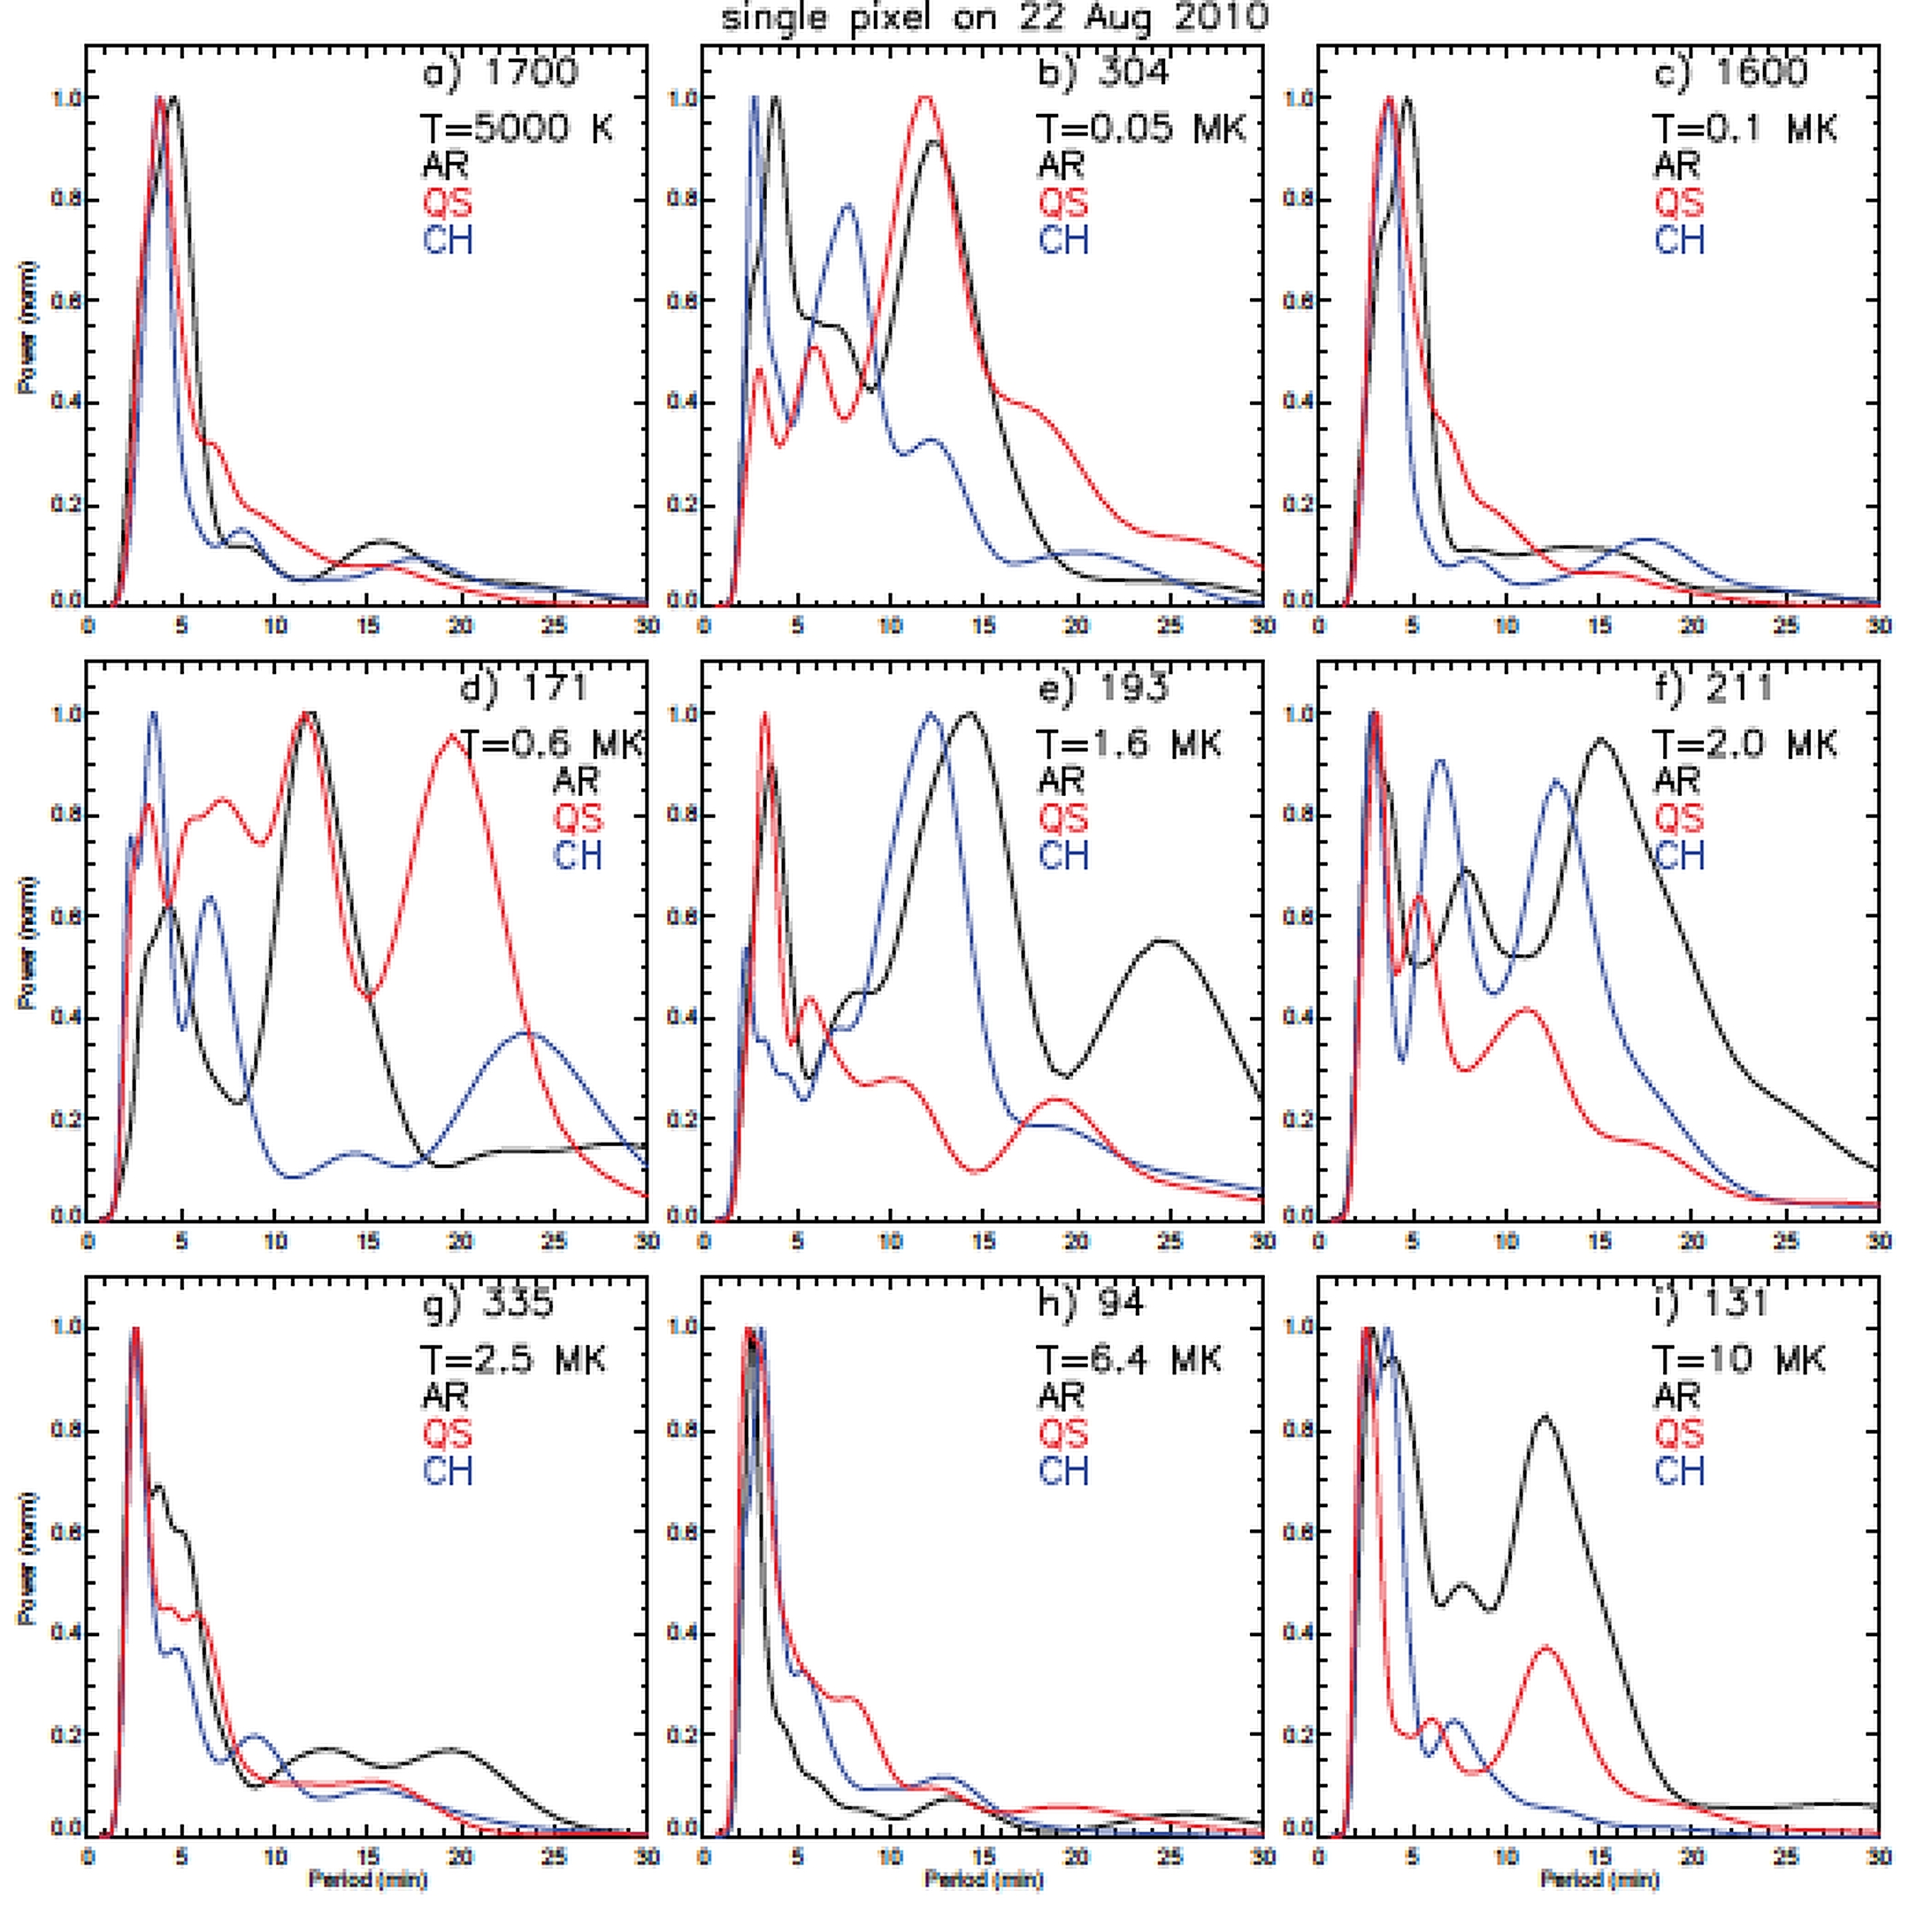
\includegraphics[scale=0.7]{imrescale/powerspectra.png}
\caption{The power spectrum in nine AIA passbands for single pixels in AR (black solid), QS (red solid), and CH (blue solid). }
\end{figure}


 The power spectra are derived by studying image sequences at solar minimum for the different solar regions e.g. AR, a typical region in QS quiet sun and a CH. The power spectra reveal strong 3-5-minute oscillations in all channels and include some longer period modes too. These results demonstrate the ubiquity of the observed 3- and 5-minute oscillations in all channels and regions and may serve as evidence of a global excitation mechanism. These observations are our strong motivation to model whether global $p$-modes may penetrate in the atmosphere. 

Previously, SDO 171$\AA$ and 193$\AA$ data were also used by \citet{Ireland2015} to compute the Fourier power spectra in the solar corona. By analysing wave propagation in four regions of the solar atmosphere with different characteristics, they found that the distribution obeys a power law at low frequencies and possesses a flat distribution at high frequencies. This contrasts with the idea of a Gaussian noise distribution and a long time-scale background. The implication is that this is the result of solar atmospheric energy propagation from elsewhere by small energy deposition events.

Evidence for the upward propagation of acoustic wave with increasing amplitude has been demonstrated through studies of variation in the intensities of chromospheric lines, for example the Ca lines at 854 nm, see  \citet{Beck2012}. Although the 
observed variations are unlikely to provide temperature rises well-known in the chromosphere they are a clear indication of the increase in dynamical activity from the photosphere to the chromosphere. The analysis of observations by  \citet{Bello2009} finds that at a height of 250 km there is an acoustic energy flux of $3000 \,W/m^2$,  2/3 of this energy is propagated by waves in the frequency range 5-10 mHz, the remaining third is carried by waves in the frequency range 10-20 mHz. Waves with frequencies greater than the acoustic cut-off of 190 s can contribute to the heating of the solar chromosphere. Reporting on measurements from the Fe I 5434, ${\AA}$ \citet{Bello2010A} detected waves with periods down to 40 s. For periods below the cut-off of 190 s 40\% of wave detections are above granules the remaining 60\% are above the intergranules. The reported best estimate of the energy flux above granules is around $3000 \, W/m^2$ whilst above the intergranules it is around $955 \, W/m^2$. Most of the acoustic flux is found between 110 s and 193 s.

Using the IMAX instrument on the Sunrise observatory, \citet{Roth2010}  reported evidence for the excitation of solar acoustic oscillations excited by turbulent flows  in the dark intergranular lanes.  Individual sunquakes with epicentres near the solar surface and located in the intergranular lanes, are assumed to feed continuously energy into the resonant $p$-modes of the Sun and provide sources for acoustic oscillations. \citet{Roth2010} presents wavefronts rippling near a granule and oriented along the direction of the intergranular lane. Using simultaneous observations of the Na and K lines with Doppler measurements, \citet{Jefferies2006} shows that inclined magnetic field lines provide portals along which magneto-acoustic energy can propagate at the intergranular boundaries.

There is a large body of computational work already undertaken to understand the propagation of waves in the solar atmosphere. Previous work, e.g. \citet{Erdelyi2007}, has considered point source drivers with a gaussian velocity distribution. Later, \citet{Fedun2009} studied the oscillatory response of the 3D solar atmosphere to the leakage of photospheric motion results are discussed in detail. High-frequency waves are shown to propagate from the lower atmosphere across the transition region, experiencing relatively low reflection, and transmitting most of their energy into the corona. It is also observed that the thin transition region becomes a wave guide for horizontally propagating surface waves for a wide range of driver periods, and particularly at those periods that support chromospheric standing waves. Additionally, the magnetic field acts as a waveguide for both high- and low-frequency waves originating from the photosphere and propagating through the transition region into the solar corona.  Other work, e.g.  \citet{Murawski2010}, has demonstrated that a strong initial pulse may lead to the quasi periodic rising of chromospheric material into the lower corona in the form of spicules, see also e.g. \citet{Khomenko2013}. \citet{Kalkofen2010}, considered the propagation of acoustic modes in a stratified hydrodynamical model of the solar atmosphere with a cylindrically symmetric driver of diameter 1Mm, they conclude that for driving regions of sizes smaller than the atmospheric scale height they are able to reproduce expansion waves which are similar to chromospheric bright points. With a weak horizontal magnetic field, the physics within the interior of supergranulation cells \citet{Lites2008} is suitably simple for undertaking hydrodynamic modelling. The modes modelled in this paper are mimicking global eigenmodes, the coherence length of eigenoscillations at the photosphere is 4 Mm, and the power peaks at 5 mins. 

\section{Numerical Computation Methods}

The 3D numerical simulations described here were undertaken using Sheffield MHD Accelerated Using GPUs \citep[SMAUG,][]{Griffiths2015}, the GPU implementation of the Sheffield Advanced Code \citep[SAC,][]{Shelyag2008}. SAC and SMAUG are numerical MHD solvers allowing us to model the time-dependent evolution of photospheric oscillations in the solar atmosphere. SAC is a derivative of the versatile advection code (VAC) developed by \citep{Toth1996}.  The general system of ideal MHD equations are
\begin{eqnarray}
&& {{\partial \rho}\over{\partial t}}+\nabla\cdot\left( \rho{\mathbf v}\right)=0, \label{e1} \\
&& {{\partial ( \rho {\bf v})}\over{\partial t}}+\nabla\cdot\left( {\bf v}\rho {\bf v}-{\bf B B}\right)+\nabla p_t=\rho{\bf g}, \label{e2}\\
&& \frac{\partial e}{\partial t}+\nabla\cdot\left({\bf v}e-{\bf B B}\cdot{\bf v}+{\bf v}p_{t}\right)+\nabla p_t=\rho{\bf g}\cdot{\bf v}, \label{e3} \\
&& {{\partial{\bf B}}\over{\partial t}} +\nabla \cdot\left(  {\bf vB}-{\bf Bv}\right)=0. \label{e4}
\end{eqnarray}
Here, $\rho$ is the mass density, $\mathbf v$ is the velocity,  $\mathbf B$ is the magnetic field, $\it{e}$ is the energy density, $p_{t}$ is the total pressure and $\mathbf g$ is the gravitational acceleration vector.
The total pressure $p_{t}$ is written as
\begin{equation}
p_{t}=p_{k}+{{\bf B}^{2}\over{2}}, \label{e5}
\end{equation}
where $p_k$ is the kinetic pressure given by
\begin{equation}
p_{k}=\left(\gamma -1\right)\left(e-\frac{\rho {\mathbf v}^{2}}{2}-\frac{{\mathbf B}^{2}}{2}\right). \label{e6}
\end{equation}
Equations (\ref{e1}) - (\ref{e6}) are applicable to an ideal compressible plasma. The SAC code is based on perturbed versions of these equations, thus the variables $\rho $, $e$ and  $\mathbf B$ are expressed in terms of perturbed and background quantities as
\begin{eqnarray}
&& \rho = \tilde{\rho}+\rho_b, \nonumber \\
&& e = \tilde{e}+e_b,  \nonumber \\
&& {\mathbf B} = \tilde{\mathbf B}+{\mathbf B}_b.  \nonumber 
\end{eqnarray}
where $\tilde{\rho}$ is the  perturbed density,  $\tilde{e}$ is the perturbed energy and $\tilde{\bf B}$  is the perturbed magnetic field. The background quantities with a subscript $\it{b}$ do not change in time, as we assume a magneto-hydrostatic equilibrium of the background plasma. 

The SMAUG code is a fully non-linear MHD numerical finite element solver for simulating, linear and non-linear wave propagation in strongly magnetised plasma with structuring and stratification. The solver applies a fourth order central differencing technique to the spatial derivatives and the Euler or fourth order Runge-Kutta method to solve the temporal derivatives. By virtue of their symmetry, central differencing schemes are conservative, with the desired side effect that the solver conserves the divergence of the magnetic field. The application of central differencing to hyperbolic differential equations results in unstable solutions with a spurious oscillatory behaviour.  Hyper-diffusion and hyper-resistivity are implemented to achieve numerical stability of the computed solution of the MHD equations \citep[see for example][]{Caunt2001}.  The primary purpose of the diffusion terms is to compensate for the anti-diffusion from truncation errors arising in the computation of temporal and spatial derivatives. When the diffusion is correctly tuned the resulting evolution is non-diffusive. In addition, the diffusion terms control the steepness of shocks by becoming large wherever the compression is large. The full set of MHD equations, including the hyper-diffusion source terms are given in \citet{Griffiths2015} and \citet{Shelyag2008}.

\section{Computational Model}

With the magnetic-field-free quiet Sun in mind, we set $\vec{B}=0$ in the MHD equations.  The computational box used for our simulations represents a volume of the solar atmosphere  with dimensions $L_{ x}= 4$ Mm and $L_{y} =4$ Mm. The model utilises a representation of the solar atmosphere with gravitational stratification in the $z$-direction and with a height of $L_{z} =6$ Mm. The computational box comprises an array of elements of dimension $128 \times 128 \times 128$. The upper boundary of our model  is in the solar corona and the lower boundary in the photosphere. The SMAUG code is well suited for modelling the leakage of wave energy from the photosphere, through the transition region and into the corona. We used open boundary conditions for the lower and upper boundaries which allowed us to model wave propagation for time scales characterised by the 5-minute $p$-mode induced oscillations. The computational model is excited by an extended vertical velocity driver located at the photosphere, this acoustic $p$-mode driver excites waves which propagate into a realistic 3D model of the solar atmosphere. In the following two sections we describe the solar atmospheric model and the implementation of the driver. 

\section{Solar Atmospheric Model}
To simulate oscillatory phenomena in the solar corona a physically representative model of the solar atmosphere is needed. 
\begin{figure}[h]
\begin{center}
\mbox{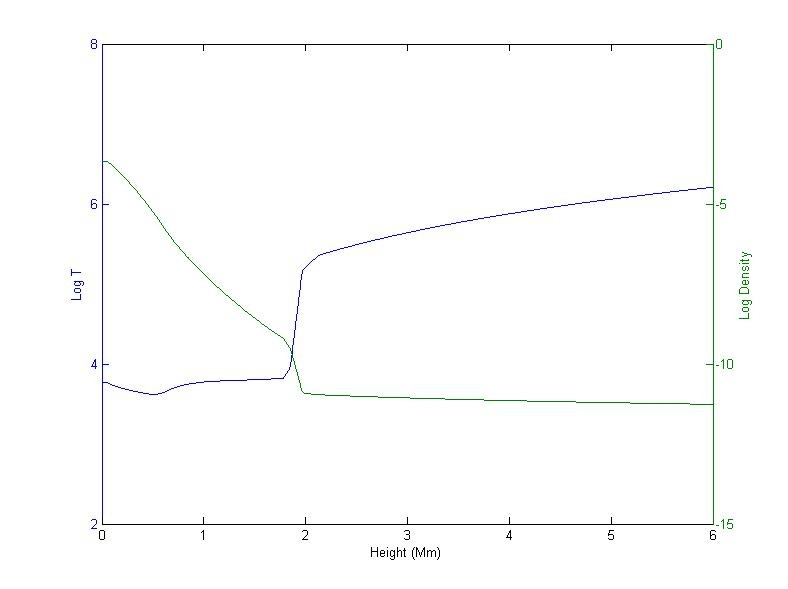
\includegraphics[scale=1]{imrescale/VAL3C_rho_temp_fig1L.jpg}}  
\mbox{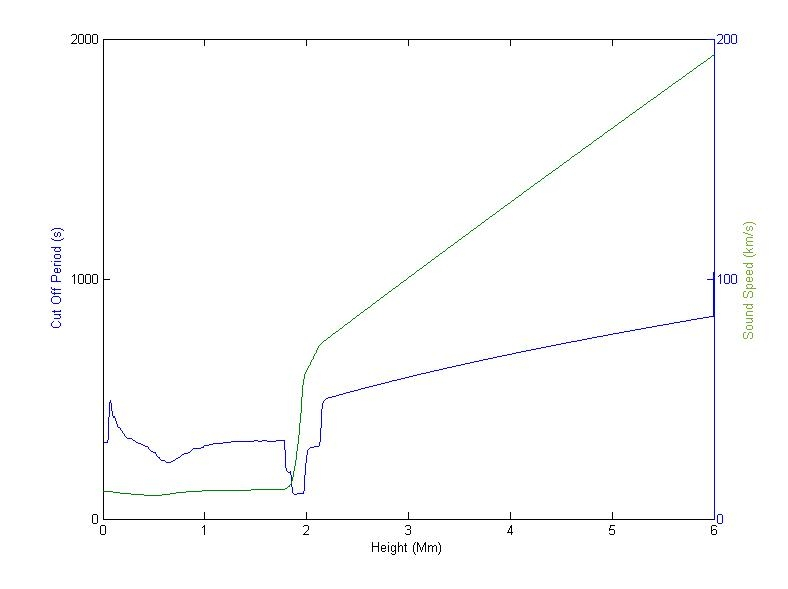
\includegraphics[scale=1]{imrescale/soundspeedVAL3C_profile_fig1R.jpg}}
\par
\end{center}
\caption{Temperature and density profiles (left) used for the model atmosphere and cut-off frequency at different heights (right).}
\label{Fig1}
\end{figure}
An option is the use of a parametrisation of the temperature of the solar atmosphere which may be a smoothed step 
function profile see \citet{Murawski2010}. Results have demonstrated the need for observationally derived semi-empirical 
models of the solar atmosphere. There is much discussion about model validity and the work undertaken to 
demonstrate the reliability of the assumptions used to construct realistic models of the solar chromosphere, see \citet{Carlsson1995}, \citet{Kalkofen2012}. The contention arises from the dynamical nature of the solar chromosphere; for example local dynamo action has been suggested as a mechanism of Joule heating in the solar chromosphere, see \citet{Leenaarts2011}. The model atmosphere employed here is an observationally derived semi-empirical representation of the quiet sun. With the fundamental assumption of hydrostatic equilibrium a model of the chromosphere in equilibrium is constructed using the VALIIIc model, see \citet{Vernazza1981}. For the region of the solar atmosphere above 2.5 Mm the results of the energy balance model of solar coronal heating has been used \citep[see][]{McWhirter1975}, his model includes an acoustic contribution comparable to the hydrostatic pressure. The corresponding temperature and density profiles are shown in Figure (\ref{Fig1}).

\section{Numerical Drivers for $p$-mode Oscillations}
For this study, the model requires a driver mimicing the solar global oscillations.  The overview of observational studies identified a range of physical phenomena resulting in oscillatory behaviour and delivering energy into the solar atmosphere.  The results presented here extend earlier work undertaken by  \citet{Malins2007A}, for their study, point drivers were used to represent periodic buffeting of turbulent motions in the photosphere. The results of the study demonstrated surface wave 
phenomena and structures in the transition region. The study highlighted the characteristics of the oscillatory 
phenomena as a result of frequency cut-offs induced by the stratified solar atmosphere. For the simulations presented in this paper, 
in contrast to the earlier models, the whole boundary of the model was perturbed.  In the real Sun, photospheric $p$-mode 
oscillations have a horizontal wavelength and coherence. Here, these excitations are represented with a 
vertical velocity driver located at the photosphere, his acoustic $p$-mode driver excites waves which propagate 
into a realistic 3D model of the solar atmosphere. Drivers representing different modes are considered, for 
example  an extended driver with a sinusoidal dependence and a wavelength of 8 Mm applied along the 
middle of the base of a computational domain of dimension 4 Mm represents  a {\it fundamental mode}. 
A driver with wavelength 4 Mm applied the same way represents the {\it first harmonic} and {\it second harmonic} 
with wavelength 2 Mm was also considered. Drivers may be constructed as an ensemble of these solar 
global eigenmodes.  Such a driver may be represented 
by an Equation (\ref{e8}) such as  
\begin{equation}
V_{z}=A_{nm} \sin\left(\frac{2\pi t}{T_s} \right)\sin\left(  \frac{(n+1)\pi x}{L_x} \right)  \sin\left(\frac{(m+1)\pi y}{L_y} \right)
\exp\left( -\frac{(z-z_0)^2}{\Delta z^2} \right),
\label{e8}
\end{equation}
In equation (\ref{e8}) $L_{x}$ and $L_{y}$ are the lengths of the base of the simulation box in the $x$ and $y$ directions respectively. $T_{s}$ is the period and $A_{nm}$ is the amplitude of the driver, the indices $n$ and $m$ define the mode. $\Delta z$ is the width of the driver which was set here to $4km$, the parameter $z_{0}$ was set so that the vertical driver location is coincident with the location of the temperature minimum which is 0.5 Mm above the lower boundary of the model i.e. the photosphere.   Since we are investigating the leakage of energy into the solar atmosphere, for consistency, it is necessary to ensure that for the different modes the driver amplitude is set to a value which provides the same total amount of energy over the model cross section and per unit time. For the $n$, $m$ mode the energy, $E_{nm}$ as a function of $z$ and time may be written as;
\begin{equation}
E_{nm}(z,t)= \rho A_{nm}^{2} I_{nm}  \sin{\left(\frac{2\pi t}{T_s} \right)}^2
\exp{\left( -\frac{(z-z_0)^2}{\Delta z^{2}} \right)}^2,
\label{e9}
\end{equation}
where $I_{nm}$ is
$$
I_{nm}= \int_{-L_{x}}^{L_{x}} \int_{L_{y}}^{+L_{y}} \sin{\left(\frac{(n+1)\pi x}{L_x} \right)}^{2}   \sin{\left(  \frac{(m+1)\pi y}{L_y} \right)}^{2}dxdy. 
$$
It is necessary to determine the amplitude $A_{mn}$ for the different modes $n, m$ with driver period 
$T_{s}$. This is achieved by computing the membrane energy integrated over the surface area and 
over a period of time from $t=0$ to $t=T_{m}$ where $T_m$ will correspond to the period of the driver 
with the largest value for the period. Following  \citet{Leighton1960}, for the fundamental mode with 
driver period 300 $s$, we set $A_{00}$=350\, ms$^{-1}$. 
Using Equation (\ref{e9}) to derive the ratio of the membrane energy for the mode $n, m$ with 
driver period $T_{s}$, the mode $(0, 0)$ with driver period $T_{00}$ and making $L_x=L_y$ 
gives the relation
\begin{equation}
A_{nm}^{2}=\frac{2A_{00}^{2}}{(n^2+m^2+2(n+m)+2)}T_{rat},
\label{e10}
\end{equation}
where $T_{rat}$ is
$$
T_{rat}=
\frac{T_m-\frac{T_{00}}{4\pi}   \sin(\frac{4\pi T_m}{T_{00}})    }{T_m-\frac{T_{s}}{4\pi}   \sin(\frac{4\pi T_m}{T_{s}})}. 
$$
This relation was used to determine the amplitudes for the higher order modes, starting from the $A_{00}$ mode we used  $A_{00}=350\, ms^{-1}$.

\section{Numerical Analysis}

Hydrodynamic simulations have been undertaken for a selection of drivers covering a range of time periods, modes and amplitudes supplying the same amount of energy, see Equation (\ref{e9}). For this investigation we have been guided by the requirement that  different driver modes deliver the same total amount of energy 
over the model cross section and when integrated over a time interval corresponding to the period of the longest period driver used for the set of simulations. With the objective to analyse and understand the nature of the energy propagation of the different modes and driver frequencies we consider a number of cases.   Three sets of simulations have been considered. Set (A) are the drivers selected because of their period, Set (B) and (C) are series of normal modes, set (C) are normal modes with equal mode numbers (see Table (\ref{Table1})). The driver periods for the normal modes are determined using the mode numbers, a value for the speed of sound (see table (\ref{Table2})) and equation (\ref{e11}). The amplitudes for each of the modes are determined by using  Equation (\ref{e10}). To use this relation, we assume 
that the $(0, 0)$ mode for the 300 s driver has an amplitude of 350 m/s \citep[see][]{Leighton1960}.
\begin{table}
\centering
\begin{tabular}{c c }
\hline
set   &  description\\
\hline
A &  Modes for the 30, 180 and 300 s driver. \\
\hline
B &  Normal Modes corresponding to different values of $c_s$ \\
\hline
C & Normal Modes for equal mode values (i.e. $n=m$)  \\
\hline
\end{tabular} 
\caption{Sets of simulations used to characterise oscillatory motions arising from an extended photospheric driver.}
\label{Table1}
\end{table}
The driver periods for Set (A) correspond to the dominant atmospheric modes of oscillation, for example, the 5-minute mode and the 3-minute chromospheric mode. The 30 s driver was selected because this corresponds to a frequency below that of the atmospheric cut-off and we can use the propagation characteristics as a test of our simulations. The periods for the normal modes were determined for different values of the speed of sound ($c_s$) in the solar atmosphere at different heights. The periods for the resulting drivers are shown in Tables (\ref{Table2})  ,   (\ref{Tableamps_equalmodenumber}) and (\ref{Tableamps_30_180_300}) .
\begin{equation}
\omega_{nm}^{2}= 2\left(\frac{\pi c_{s}}{L} \right)^{2},
\label{e11}
\end{equation}

where $L$ is the box length.
\begin{table}
\centering
\begin{tabular}{c c c }
\hline
Mode &  $20$ km/s &  $
31.4$ km/s \\
\hline
0,0  & 282.8 & 180.0 \\
\hline
0,1  & 200.0 & 127.3  \\
\hline
0,2  & 133.3 & 84.8  \\
\hline
0,3  & 100.0 & 63.6  \\
\hline
\end{tabular} 
\caption{The table shows the driver periods used for different wave modes. The first mode number corresponds to the mode for the $x$-direction and the second number the mode for the $y$-direction. The table corresponds to the normal modes labelled set B. The table column headings show the value of the speed of sound, $c_s$, computed for the normal modes using equation \ref{e11}. }
\label{Table2}
\end{table}

%this table is notpresent in text !
\begin{table*}\label{simcperiods}
\centering
\begin{tabular}{c c }
\hline
Mode   &  Period (s) \\
\hline
1,1 & 471.4  \\
\hline
2,2 & 235.7   \\
\hline
3,3 & 157.1   \\
\hline

\end{tabular} 
\caption{The table shows the driver periods used for different wave modes. The first mode number corresponds to the mode for the $x$-direction and the second number the mode for the $y$-direction. The table corresponds to the normal modes labelled set C. The table column headings show the value of the speed of sound, $c_s$, computed for the normal modes using equation \ref{e11}.}
\label{Tableamps_equalmodenumber}
\end{table*}

%this table is notpresent in text !
\begin{table*}\label{simamps}
\centering
\begin{tabular}{c c c c }
\hline
Mode   & 30 s driver amplitude & 180 s s driver amplitude & 300 s s driver amplitude\\
\hline
0,0 & 343.4 & 348.3 & 350.0 \\
\hline
0,1 & 217.2 & 220.3 & 221.4 \\
\hline
0,2 & 153.6 & 155.8 & 156.5 \\
\hline
0,3 & 117.8 & 119.5 & 120.0 \\
\hline
\end{tabular} 
\caption{The table shows the driver amplitudes used for different wave modes. The first mode number corresponds to the mode for the $x$-direction and the second number the mode for the $y$-direction. The table corresponds to the modes labelled set A. The table column headings show the driver period each table entry shows the amplitude computed using equation \ref{e10}.}
\label{Tableamps_30_180_300}
\end{table*}






%This table DOES not have \label i.e. NOT shown in text !
\begin{table*}[h]
\centering
\begin{tabular}{c c c c c }
\hline
   &  1 Mm & 2 Mm & 4 Mm & 5.5 Mm \\
\hline
30 &  0.0133 & 1.7275x$10^{-4}$ & 1.0561x$10^{-4}$ & 5.5399x$10^{-5}$ \\
\hline
300 & 0.2607 & 0.008144 & 0.002176 &  0.001119 \\
\hline
180 & 0.7227 & 0.047895 & 0.019831 &  0.010365 \\
\hline
435.1 & 1.9415 & 0.043601 & 0.005944 & 0.003147  \\
\hline
179.98 & 1.6450 & 0.004502 & 0.002600&  0.001366 \\ 
\hline
%282.84 & 0.1986 & 0.004007 & 0.001845 &  9.7821x$10^{-4}$ \\
\hline
\end{tabular} 
\caption{ $(0, 0)$ mode energy ratio, the energy is the ratio of the energy flux at a given height to the energy flux at the location of the driver.}
\label{Table00mode}
\end{table*}

%This table DOES not have \label i.e. NOT shown in text !
\begin{table*}[h]
\centering
\begin{tabular}{c c c c c }
\hline
   &  1 Mm & 2 Mm & 4 Mm & 5.5 Mm \\
\hline
30 &  0.0065 & 1.751x$10^{-5}$ &  1.2579x$10^{-6}$ & 4.6820x$10^{-7}$ \\
\hline
300 & 0.1001 & 8.796x$10^{-4}$ &  4.1494x$10^{-6}$ &  1.3059x$10^{-6}$ \\
\hline
180 & 0.1543 &  5.8381x$10^{-4}$ &  3.2715x$10^{-5}$ &  1.1343 x$10^{-5}$ \\
\hline
307.1 & 0.0982 & 0.001 & 4.1351x$10^{-6}$ & 1.3380 x$10^{-6}$  \\
\hline
127.27 & 0.0829 &  4.3190x$10^{-4}$ &  5.1387x$10^{-5}$ & 2.0397 x$10^{-5}$ \\ 
\hline
200.0 & 0.1126 &  4.4180x$10^{-4}$ &  2.0186x$10^{-5}$ & 6.3062 x$10^{-6}$ \\
\hline
\end{tabular} 
\caption{ $(0, 1)$ mode energy ratio, the energy is the ratio of the energy flux at a given height to the energy flux at the location of the driver.}
\label{Table01mode}
\end{table*}

%This table DOES not have \label i.e. NOT shown in text !
\begin{table*}[h]
\centering
\begin{tabular}{c c c c c }
\hline
   &  1 Mm & 2 Mm & 4 Mm & 5.5 Mm \\
\hline
30 &  0.0024 & 7.2158 x$10^{-6}$ & 1.0651x$10^{-6}$ & 7.6079x$10^{-7}$\\
\hline
300 & 0.0578 & 4.9604 x$10^{-4}$ & 5.5618x$10^{-6}$ & 4.1907x$10^{-6}$\\
\hline
180 & 0.0687 & 3.5547 x$10^{-4}$ & 6.0675x$10^{-5}$ & 4.1492 x$10^{-5}$\\
\hline
205.1 & 0.3135 & 0.0015 &1.6520x$10^{-4}$ & 1.1272x$10^{-4}$\\
\hline
84.84 & 0.0206 &5.8903 x$10^{-5}$1.6520 x$10^{-5}$ & 1.1890 x$10^{-5}$\\
\hline
133.33 & 0.0497 & 1.9731x$10^{-4}$7.9834 x$10^{-5}$ & 5.6267 x$10^{-5}$\\
\hline
\end{tabular} 
\caption{ $(0, 2)$ mode energy ratio, the energy is the ratio of the energy flux at a given height to the energy flux at the location of the driver.}
\label{Table02mode}
\end{table*}

%This table DOES not have \label i.e. NOT shown in text !
\begin{table*}[h]
\centering
\begin{tabular}{c c c c c }
\hline
   &  1 Mm & 2 Mm & 4 Mm & 5.5 Mm \\
\hline
30 &  0.0101 &  4.2736x$10^{-5}$ & 6.3291x$10^{-7}$ & 3.7786x$10^{-7}$\\
\hline
300 & 0.0359 & 3.8929x$10^{-4}$ & 3.2621x$10^{-7}$ & 2.1259x$10^{-7}$\\
\hline
180 & 0.0351 &1.3948x$10^{-4}$ & 3.1342x$10^{-6}$ & 1.8205x$10^{-6}$\\
\hline
153.8 & 0.0313 & 1.1043x$10^{-4}$ & 3.8071x$10^{-6}$ & 2.1034x$10^{-6}$\\
\hline
63.63 & 0.0051 & 9.8989x$10^{-6}$ & 7.0207x$10^{-7}$ & 4.0621x$10^{-7}$\\
\hline
100.0 & 0.0151 & 3.0678x$10^{-5}$ & 2.8527x$10^{-6}$ & 1.6707x$10^{-6}$\\
\hline
\end{tabular} 
\caption{$(0, 3)$ mode energy ratio, the energy is the ratio of the energy flux at a given height to the energy flux at the location of the driver.}
\label{Table03mode}
\end{table*}

%This table DOES not have \label i.e. NOT shown in text !
\begin{table*}[h]
\centering
\begin{tabular}{c c c c c }
\hline
   &  1 Mm & 2 Mm & 4 Mm & 5.5 Mm \\
\hline
$(0, 0)$ &  0.7227 & 0.0479 & 0.0198 & 0.0104 \\
\hline
$(0, 1)$ & 0.1543 & 0.0006 & 3.2715x$10^{-5}$ &  1.1343x$10^{-5}$\\
\hline
$(0, 2)$ & 0.0687 & 0.0004 & 6.0675x$10^{-5}$ &  4.1492x$10^{-5}$\\
\hline
$(0, 3)$ & 0.0351 & 0.0001 & 3.1342x$10^{-6}$ & 1.8205 x$10^{-6}$\\
\hline
$(1, 1)$ & 0.4072 & 0.0011 & 4.5311x$10^{-6}$ &  5.5495x$10^{-7}$\\
\hline
$(1, 2)$ & 0.3331 & 0.0012 & 3.0728x$10^{-6}$ &  1.3055x$10^{-6}$\\
\hline
$(1, 3)$ & 0.2961 & 0.0011 & 4.8733x$10^{-7}$ &  3.4760x$10^{-7}$\\
\hline
$(2, 2)$ & 0.3054 & 0.0011 & 1.5844x$10^{-5}$ &  1.7622x$10^{-5}$\\
\hline
$(2, 3)$ & 0.2732 & 0.0008 & 2.1443x$10^{-6}$ &  1.7045x$10^{-6}$\\
\hline
$(3, 3)$ & 0.2205 & 0.0006 & 1.9711x$10^{-7}$ &  2.6756x$10^{-7}$\\
\hline
\end{tabular} 
\caption{180 s driver energy ratio, the energy is the ratio of the energy flux at a given height to the energy flux at the location of the driver.}
\label{Table180mode}
\end{table*}

%This table DOES not have \label i.e. NOT shown in text !
\begin{table*}[h]
\centering
\begin{tabular}{c c c c c }
\hline
   &  1 Mm & 2 Mm & 4 Mm & 5.5 Mm \\
\hline
$(0, 0)$ &  0.2607 & 0.0081 & 2.2x$10^{-3}$ &  1.1x$10^{-3}$\\
\hline
$(0, 1)$ & 0.1001 & 0.0009 & 4.1494x$10^{-6}$ &  1.3059x$10^{-6}$\\
\hline
$(0, 2)$ & 0.0578 & 0.0005 & 5.5618x$10^{-6}$ &  4.1907x$10^{-6}$\\
\hline
$(0, 3)$ & 0.0359 & 0.0004 &3.2621x$10^{-7}$ &  2.1259x$10^{-7}$\\
\hline
$(1, 1)$ & 0.2267 & 0.0016 & 9.9329x$10^{-7}$ &  1.0749x$10^{-7}$\\
\hline
$(1, 2)$ & 0.2535 & 0.0016 & 8.2058x$10^{-7}$ &  2.8814x$10^{-7}$\\
\hline
$(1, 3)$ & 0.2692 & 0.0023 & 2.1995x$10^{-7}$ &  9.0161x$10^{-8}$\\
\hline
$(2, 2)$ & 0.2625 & 0.0021 & 1.4846x$10^{-6}$ &  1.7399x$10^{-6}$\\
\hline
$(2, 3)$ & 0.2328 & 0.0017 & 2.4839x$10^{-7}$ &  2.0699x$10^{-7}$\\
\hline
$(3, 3)$ & 0.2036 & 0.0012 & 7.2069x$10^{-8}$ &  4.944x$10^{-8}$\\
\hline
\end{tabular} 
\caption{300 s driver energy ratio, the energy is the ratio of the energy flux at a given height to the energy flux at the location of the driver.}
\label{Table300mode}
\end{table*}








%FIGURE 5 here caption:Three-dimensional snapshots of the evolution of Vz showing the development of the initial perturbation in the nonmagnetic equilibrium generated 
%by the 30-second-period driver (in ms?1) at the times (a) t = 112 seconds, (b) t = 216 seconds, (c) t = 244 seconds, and (d) t = 316 seconds. 
%The z-axis corresponds to height measured in megameters and the x and y horizontal axes are parallel to the solar surface.\\

%\begin{figure*}[h]\label{fig5_30svz_vt_mode0}
%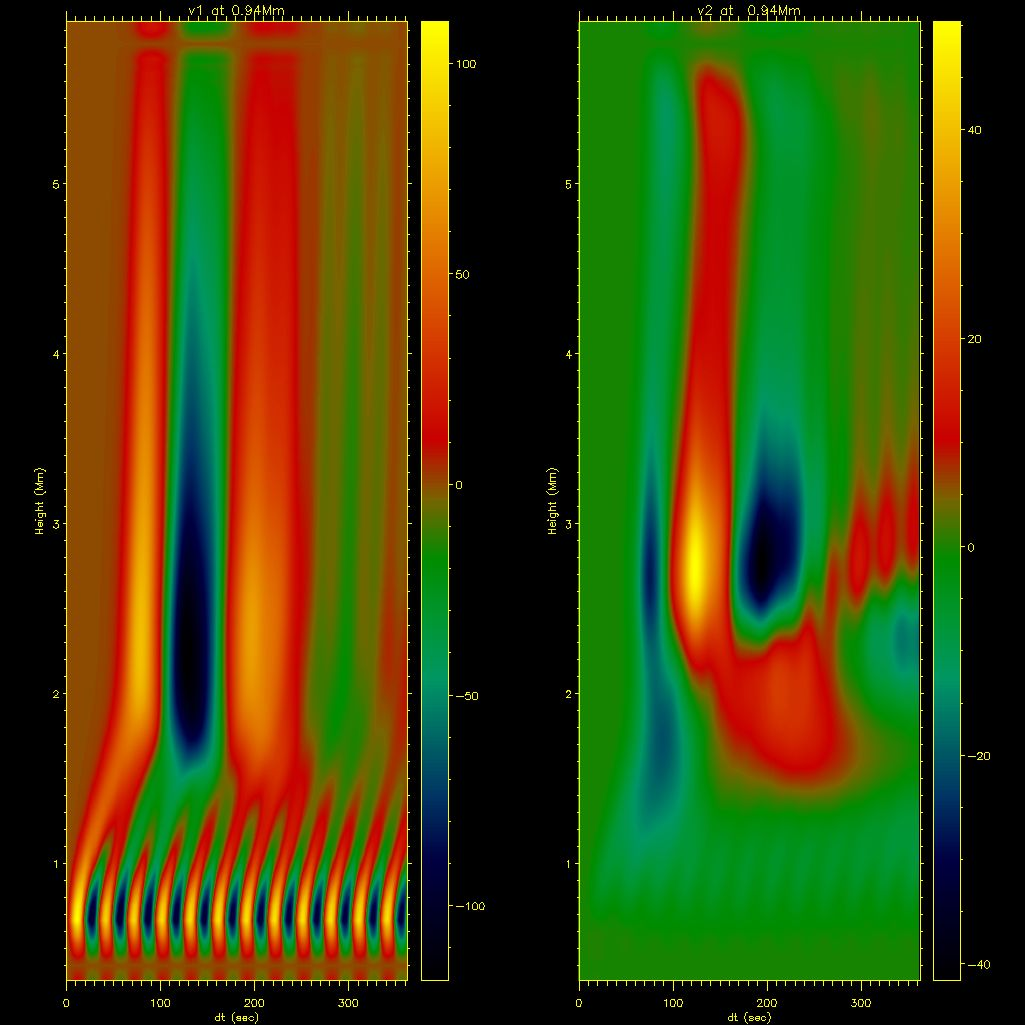
\includegraphics[scale=0.5]{images/pm30s_sindrv_n0_4b03d_dt.jpg}
%\caption{Three-dimensional snapshots of the evolution of Vz showing the development of the initial perturbation in the nonmagnetic equilibrium generated by the 30-second-period %driver (in ms?1) at the times (a) t = 112 seconds, (b) t = 216 seconds, (c) t = 244 seconds, and (d) t = 316 seconds. The z-axis corresponds to height measured in megameters and the x and y %horizontal axes are parallel to the solar surface. }
%\end{figure*}

% this table DOES NOT HAVE a \label !!!! i.e. not present in text !
%\begin{table*}
%\centering
%\begin{tabular}{cccc}
%\hline
%Label   &  Density profile & Gravity enabled & Driver \\
%\hline
%B &  VALIIC & yes & single driver at photosphere \\
%\hline
%C & VALIIC & no & single driver at photosphere \\
%\hline
%D & constant density & yes & single driver at photosphere \\
%\hline
%E & constant density & no & single driver at photosphere \\
%\hline
%F & constant density & no & two drivers at the photosphere \\ and transition zone\\
%\hline
%\end{tabular} 
%\caption{Simulations used to characterise oscillatory motions arising from the surface driver.}
%\end{table*}

\section{Results of Numerical Simulation}

The propagation of waves in a stratified atmosphere can be understood using linearised versions of the 
equation of continuity, momentum and energy. Such atmospheric waves of expansion have been 
considered for many years, initiated by e.g. \citet{Lamb1932}. Owing to the high gradients, partial 
reflection of acoustic waves at all frequencies is expected at the transition region. The transition region 
is the upper boundary of the chromospheric cavity, it has been previously suggested that this is the source 
of three-minute transition-region oscillations, see \citet{Leibacher1971}. It is known that the propagation of 
acoustic waves in an unbounded stratified medium is determined by a cut-off period. In a gravitationally 
stratified atmosphere acoustic waves can only propagate if the wave period is less than the cut-off period. 
Waves with a period greater than the cut-off are evanescent. Following \citet{Taroyan2008}, by solving the 
Klein-Gordon equation for the gravitationally stratified atmosphere i.e, 
$$
\frac{\partial^2 Q}{\partial t^2} - c_s^2(z) \frac{\partial^2 Q}{\partial z^2} + \Omega^2(z)Q = 0,
$$
the cut-off period, $P_{c}(z)$, for the atmosphere at a given height, $z$, can be obtained from:
$$
P_{c}(z)=\frac{2\Lambda_0   }{ c_{s}(z)}   \sqrt{\frac{1}{1+2\frac{d}{dz}\Lambda_0(z)}}.
$$
The pressure scale height for an atmosphere stratified by a uniform gravitational field is given by
$$
\Lambda_0(z)=\frac{p_0(z)}{g\rho_0(z)}.
$$
Here, $p_0(z)$ and $\rho_0(z)$ are the equilibrium pressure and density as a functions of height, respectively. $Q$ is the 
re-scaled perturbation of the velocity. The variation of the cut-off frequency as a function of solar atmospheric height is shown in 
Figure (\ref{Fig1}) (see right panel) which unveils the cut-off period for the case of VALIII atmosphere and isothermal 
atmosphere, respectively. It is recognised from Figure (\ref{Fig1}) that there are a number of distinct 
regions of propagation behaviour. For the photosphere, near the temperature minimum, the cut-off period is 300 s, therefore, 
it is expected that the 5 minutes modes are evanescent. In the chromosphere the cut-off period increases to a value greater than 300 s, 
therefore the five minute modes can propagate once they are either excited here or can propagate here due to e.g. leakage. For the transition zone the cut-off drops to a value which goes down to 100 s. In the corona, it is seen that a much greater range of frequencies can propagate.

To determine how wave energy propagation is influenced by the wave modes and frequencies, we compute the time averaged wave energy flux integrated over the cross-sectional area of the simulation box at different heights. The area of integration is perpendicular to the model $z$-axis.
\begin{equation}
F_{int}= \frac{1}{t_{max}} \int_{0}^{t_{max}} \int {\mathbf F}_{wave} \cdot d{\mathbf A}dt,
\label{e11}
\end{equation}
where the wave energy flux $\bf{F}_{wave}$ is given by
$$
{\mathbf F}_{wave}=\tilde{p}_{k} {\mathbf v}.
$$
The expression for the wave energy flux is dependent on the perturbed kinetic pressure, $\tilde{p}_{k}$, given by \citet{Bogdan2003}
$$
\tilde{p}_{k}=\left(\gamma - 1\right)\left( \tilde{e}-\frac{ \left( \tilde{\rho} +\rho_b \right){\mathbf v}^2}{2}\right).
$$

The full set of videos for all the simulations performed have been made publically available on the digital media repository hosted by The University of Sheffield, see \citet{Griffiths2017}. Each video shows the value of the vertical component of the plasma velocity ($z$-component) along different slices through the simulation box. The scale shows the velocity in m/s. The green vectors represent the velocity directions along a single slice through the simulation. The green surface at a height of 3.5 Mm is the 2 MK temperature isosurface. 
Each video is labelled using three numbers. The first number is the driver period in seconds. The following 2 integers are each of the mode indices for the $x$- and $y$-direction, respectively.
\begin{figure}[h]
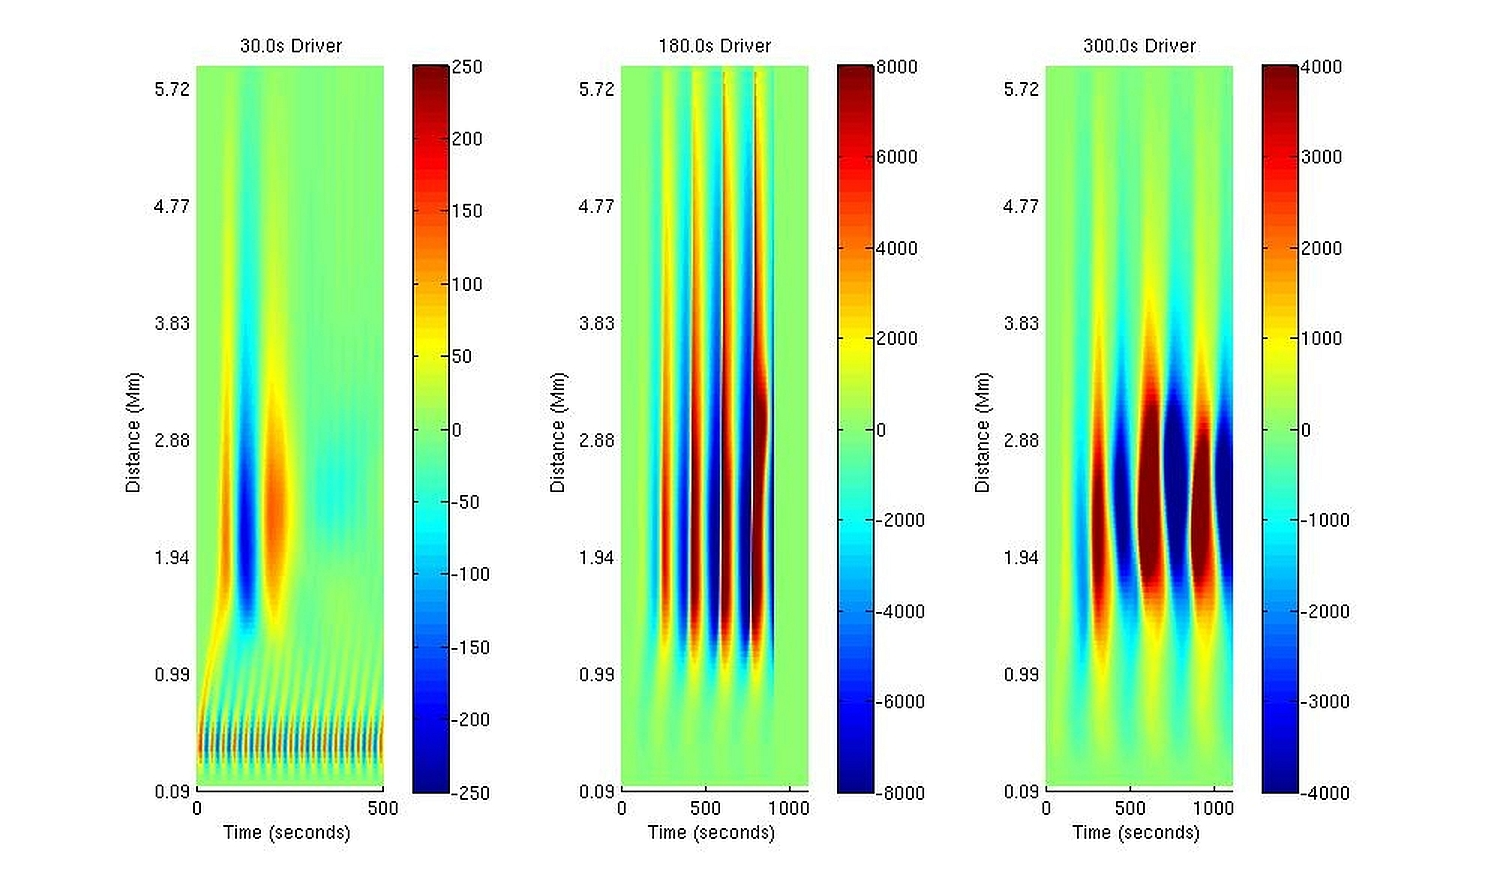
\includegraphics[scale=1.8]{imrescale/fig2_dt_30_180_300_0_vert_2Mm.jpg}
\caption{Time-distance plot for the fundamental mode $(0,0)$ and 30, 180 and 300 s driver period for the $z$ component of the velocity for a vertical slice across the box  taken at 2 Mm and shows  the profile of $v_{z}$ through the solar atmosphere for different time steps (the left hand plot shows the case for the 30 s driver, the centre plot the case for the 180 s driver and the right hand plot shows the case for the 300 s  driver). }
\label{Fig3}
\end{figure}
\begin{figure}[h]
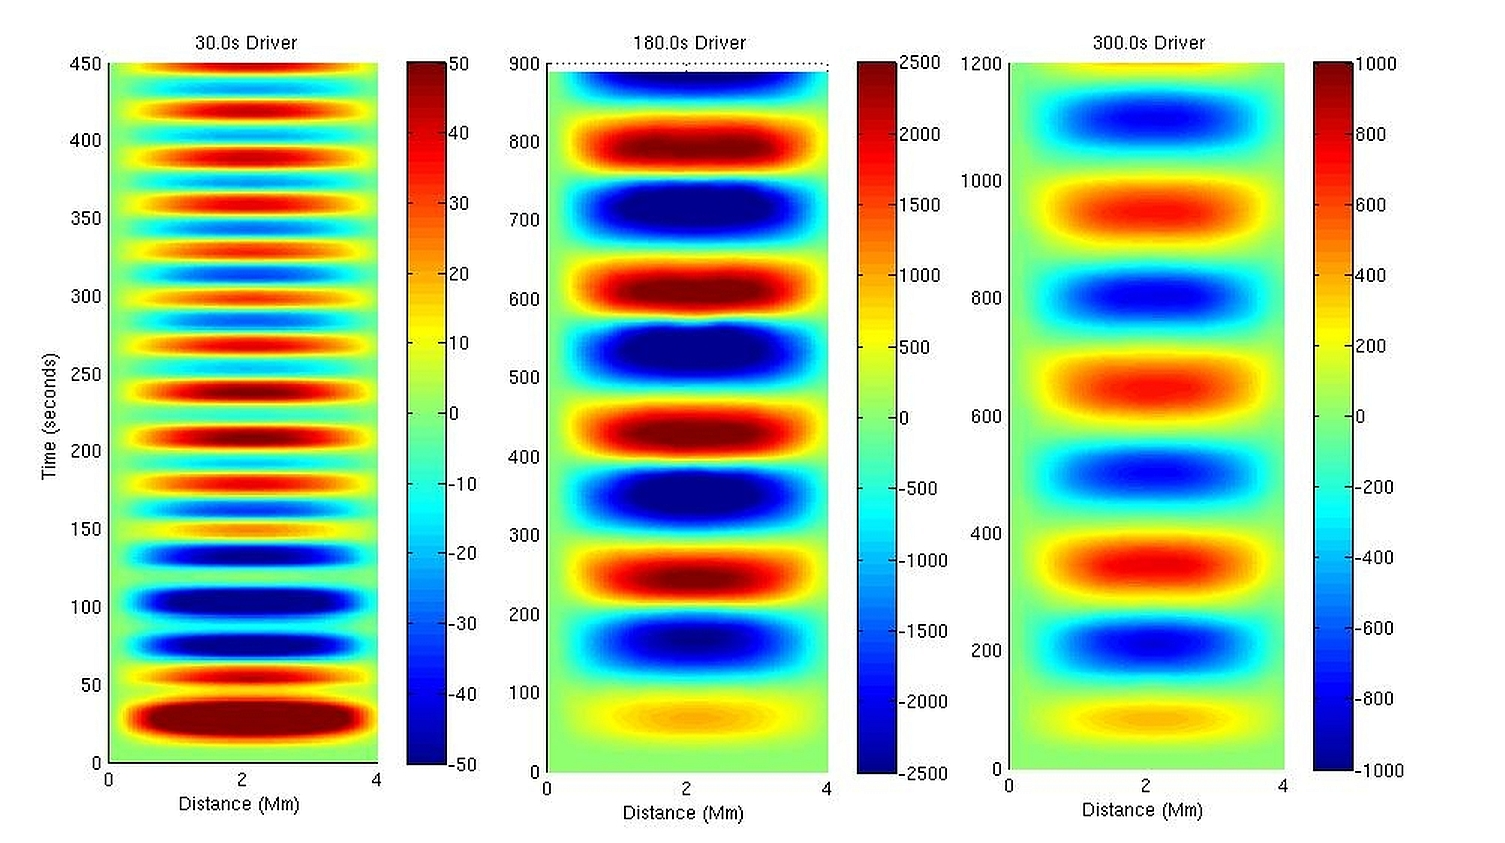
\includegraphics[scale=1]{imrescale/fig3_dt_30_180_300_0_horiz_p94Mm.jpg}
\caption{Time-distance plot for the fundamental mode $(0,0)$  and 30, 180 and 300 s driver period for the $z$ component of the velocity for a horizontal slice across the box  taken at 0.94 Mm shows  the profile of $ v_{z}$ across the simulation box at a given point (left hand is 30 s driver, centre is 180 s driver and the right hand is the 300 s driver). }
\label{Fig4}
\end{figure}
\begin{figure}[h]
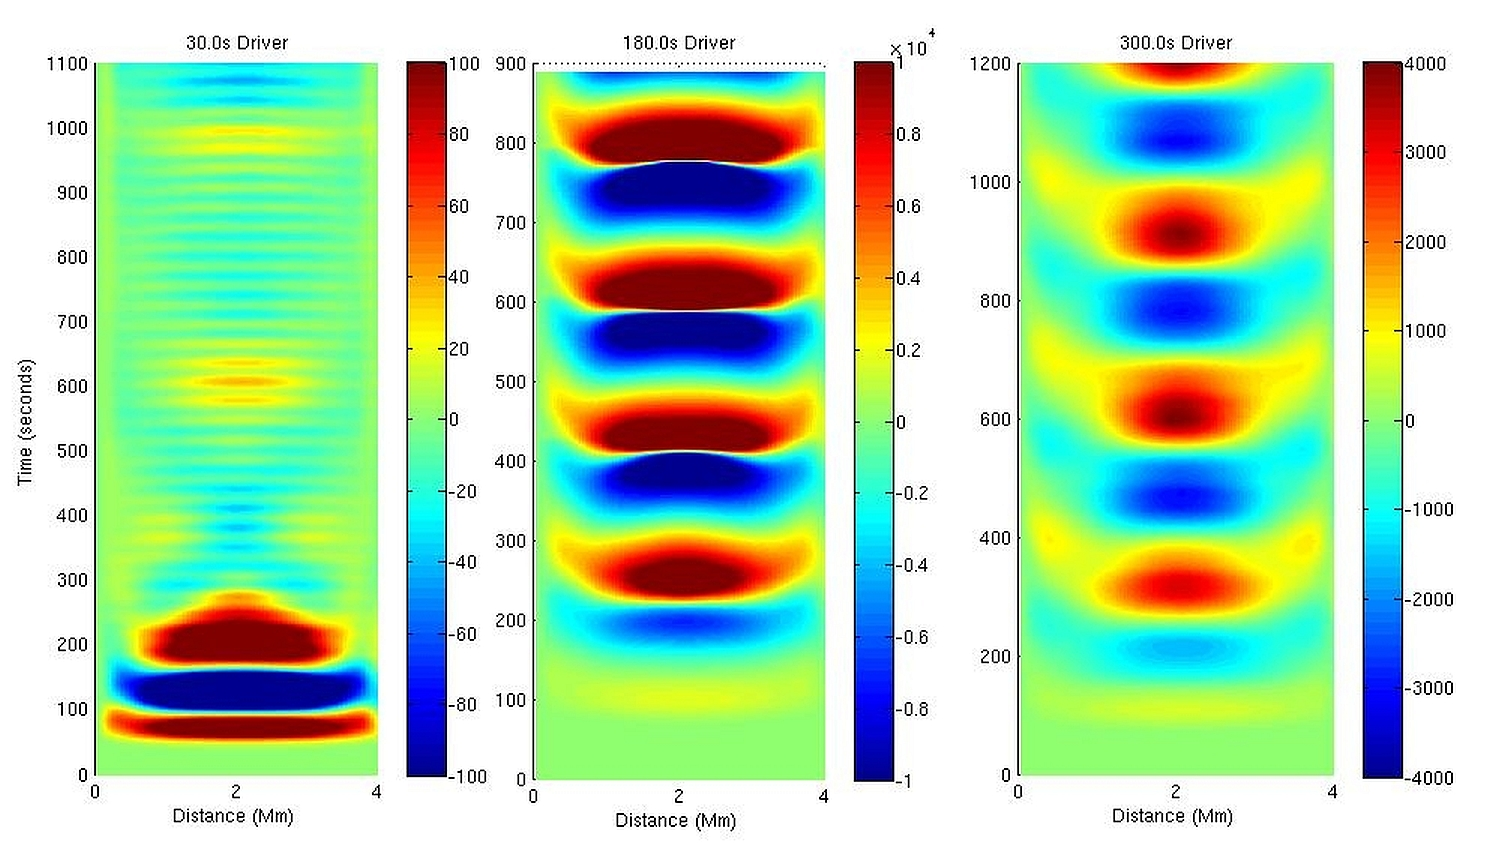
\includegraphics[scale=1]{imrescale/fig4_dt_30_180_300_0_horiz_2Mm.jpg}
\caption{Time-distance plot for the fundamental model and 30, 180 and 300 s driver period for the $z$ component of the velocity for a horizontal slice across the box  taken at the transition zone shows  the profile of $v_{z}$ across the simulation box at a height of 2 Mm (left hand is 30 s driver, centre is 180 s driver and the right hand is the 300 s driver). }
\label{Fig5}
\end{figure}
\begin{figure}[h]
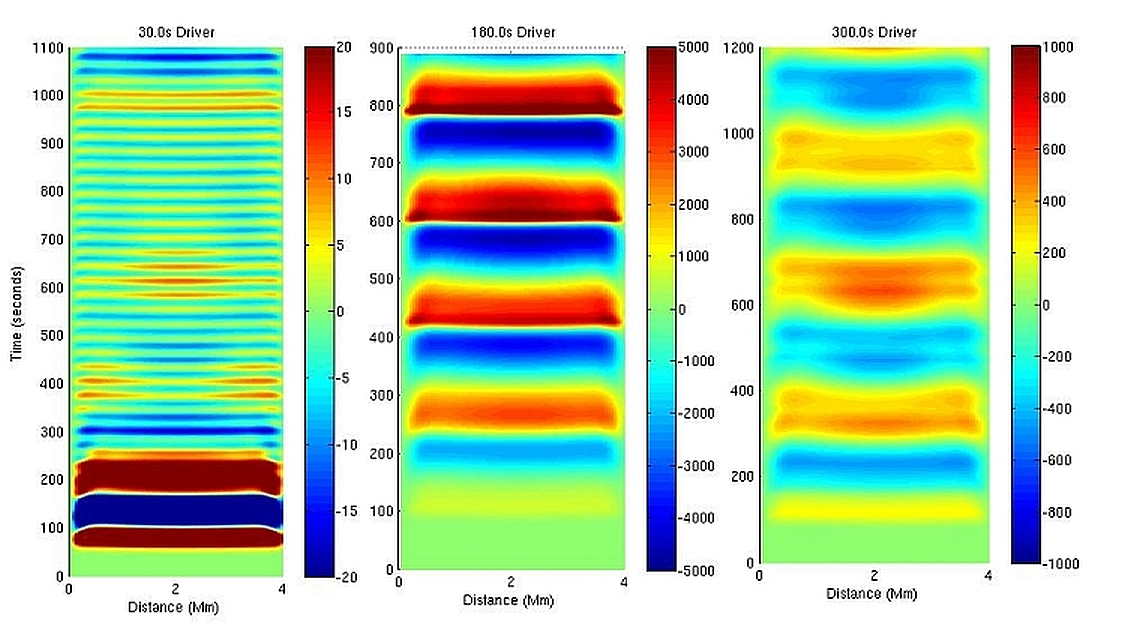
\includegraphics[scale=1]{imrescale/fig5_dt_30_180_300_0_horiz_4p2Mm.jpg}
\caption{Time-distance plot for the fundamental mode and 30, 180 and 300 s driver period for the $z$ component of the velocity for a horizontal slice across the box  taken at 4.2 Mm shows  the profile of $v_{z}$ across the simulation box (left hand is 30 s driver, centre is 180 s driver and the right hand is the 300 s driver). }
\label{Fig6}
\end{figure}
For the fundamental modes $(0, 0)$  illustrated in Figures (\ref{Fig3}-\ref{Fig6})  we observe that there is no significant structure at the transition zone. However, the 30 s mode demonstrates the rapid expansion of the perturbation at the penetration height of the the transition region. This is accompanied with an increase in the transverse velocity $(v_x)$. This observation is true for all 30, 180 and 300 s driver scenarios. As the mode order is increased from $n=0$, to $n=1$ and then $n=2$ it is observed that transition region structuring becomes apparent and is more reminiscent of the observations of \citet{Malins2007A}.

For the fundamental modes with the 30, 180 and 300 s drivers we have produced time-distance plots of the plasma velocity, $v_z$, i.e., in the same direction as the driver and in the direction of increasing height through the solar atmosphere.  Figure (\ref{Fig7})
 shows the time-distance plots for a vertical section through the simulation box. Since this was a fundamental mode the section was taken through the middle of the simulation box. The plots show that the greatest amplitude arises in the transition region, in particular for the 180 s driver. Looking at the result for the 30 s driver, it is seen that the initial travelling response reaches a response at around 0.5 Mm corresponding to a cut-off of 200 s. The maximum amplitude is coherent with the maximum occurring at the same frequency as that of the driver. For the first 70 periods, maxima appear in the transition zone. It also appears that the transition zone is essentially a source of excitation with frequency lower than that of the driver, however, at longer time periods these motions occur with reduced amplitude but with the same period as the driver. For the 180 and 300 s drivers it is observed that the amplitude in the transition zone is larger than that for the 30 s driver by a factor of up to 20. For the 30, 180 and 300 s cases we observe the travelling wave in the chromosphere and in the solar corona. Although the 180 s mode shows the greatest excitation both the 180 and 300 s drivers become evanescent due the the cut-off period for the upper atmosphere. The intensity peak for the 180s  driver is a result of the Chromospheric resonance which is well documented, see for example \citet{Fleck1991}.  Figures \ref{Fig11} and \ref{Fig14} show the time-distance plots for a horizontal section taken at a height of 0.94 Mm, i.e. through the chromosphere. The travelling modes in these plots propagate as plane modes with a frequency consistent with that of the driver. The greatest intensity is observed for the 180 s driver. Propagation for the transition zone shows the most powerful response for the 180 s driver followed by the 300 s driver. The response for the 30 s driver decays rapidly after the first ten cycles. As we move into the solar corona there is further attenuation with the greatest signal reduction for the 30 s driver.

The time-distance plots for horizontal sections are illustrated in Figures (\ref{Fig11}-\ref{Fig16}), at an atmospheric height of 4.2 Mm there is a clear indication of the propagation of waves across the transition zone. For the case of the 30 s driver it can be seen that  the propagation is cut-off after the first 270 s of the simulation. All three driver cases indicate a peak with a width of around 90 s. This peak exhibits a degree of splitting which is most clear for the 300 s driver.  This effect may be attributable to the superposition of waves reflected from the boundaries of the chromosphere.

%FIGURE 7 here caption:Time-distance plot for fundamental model with 300s period for the z  component of the velocity. x-direction\\

\begin{figure}[h]
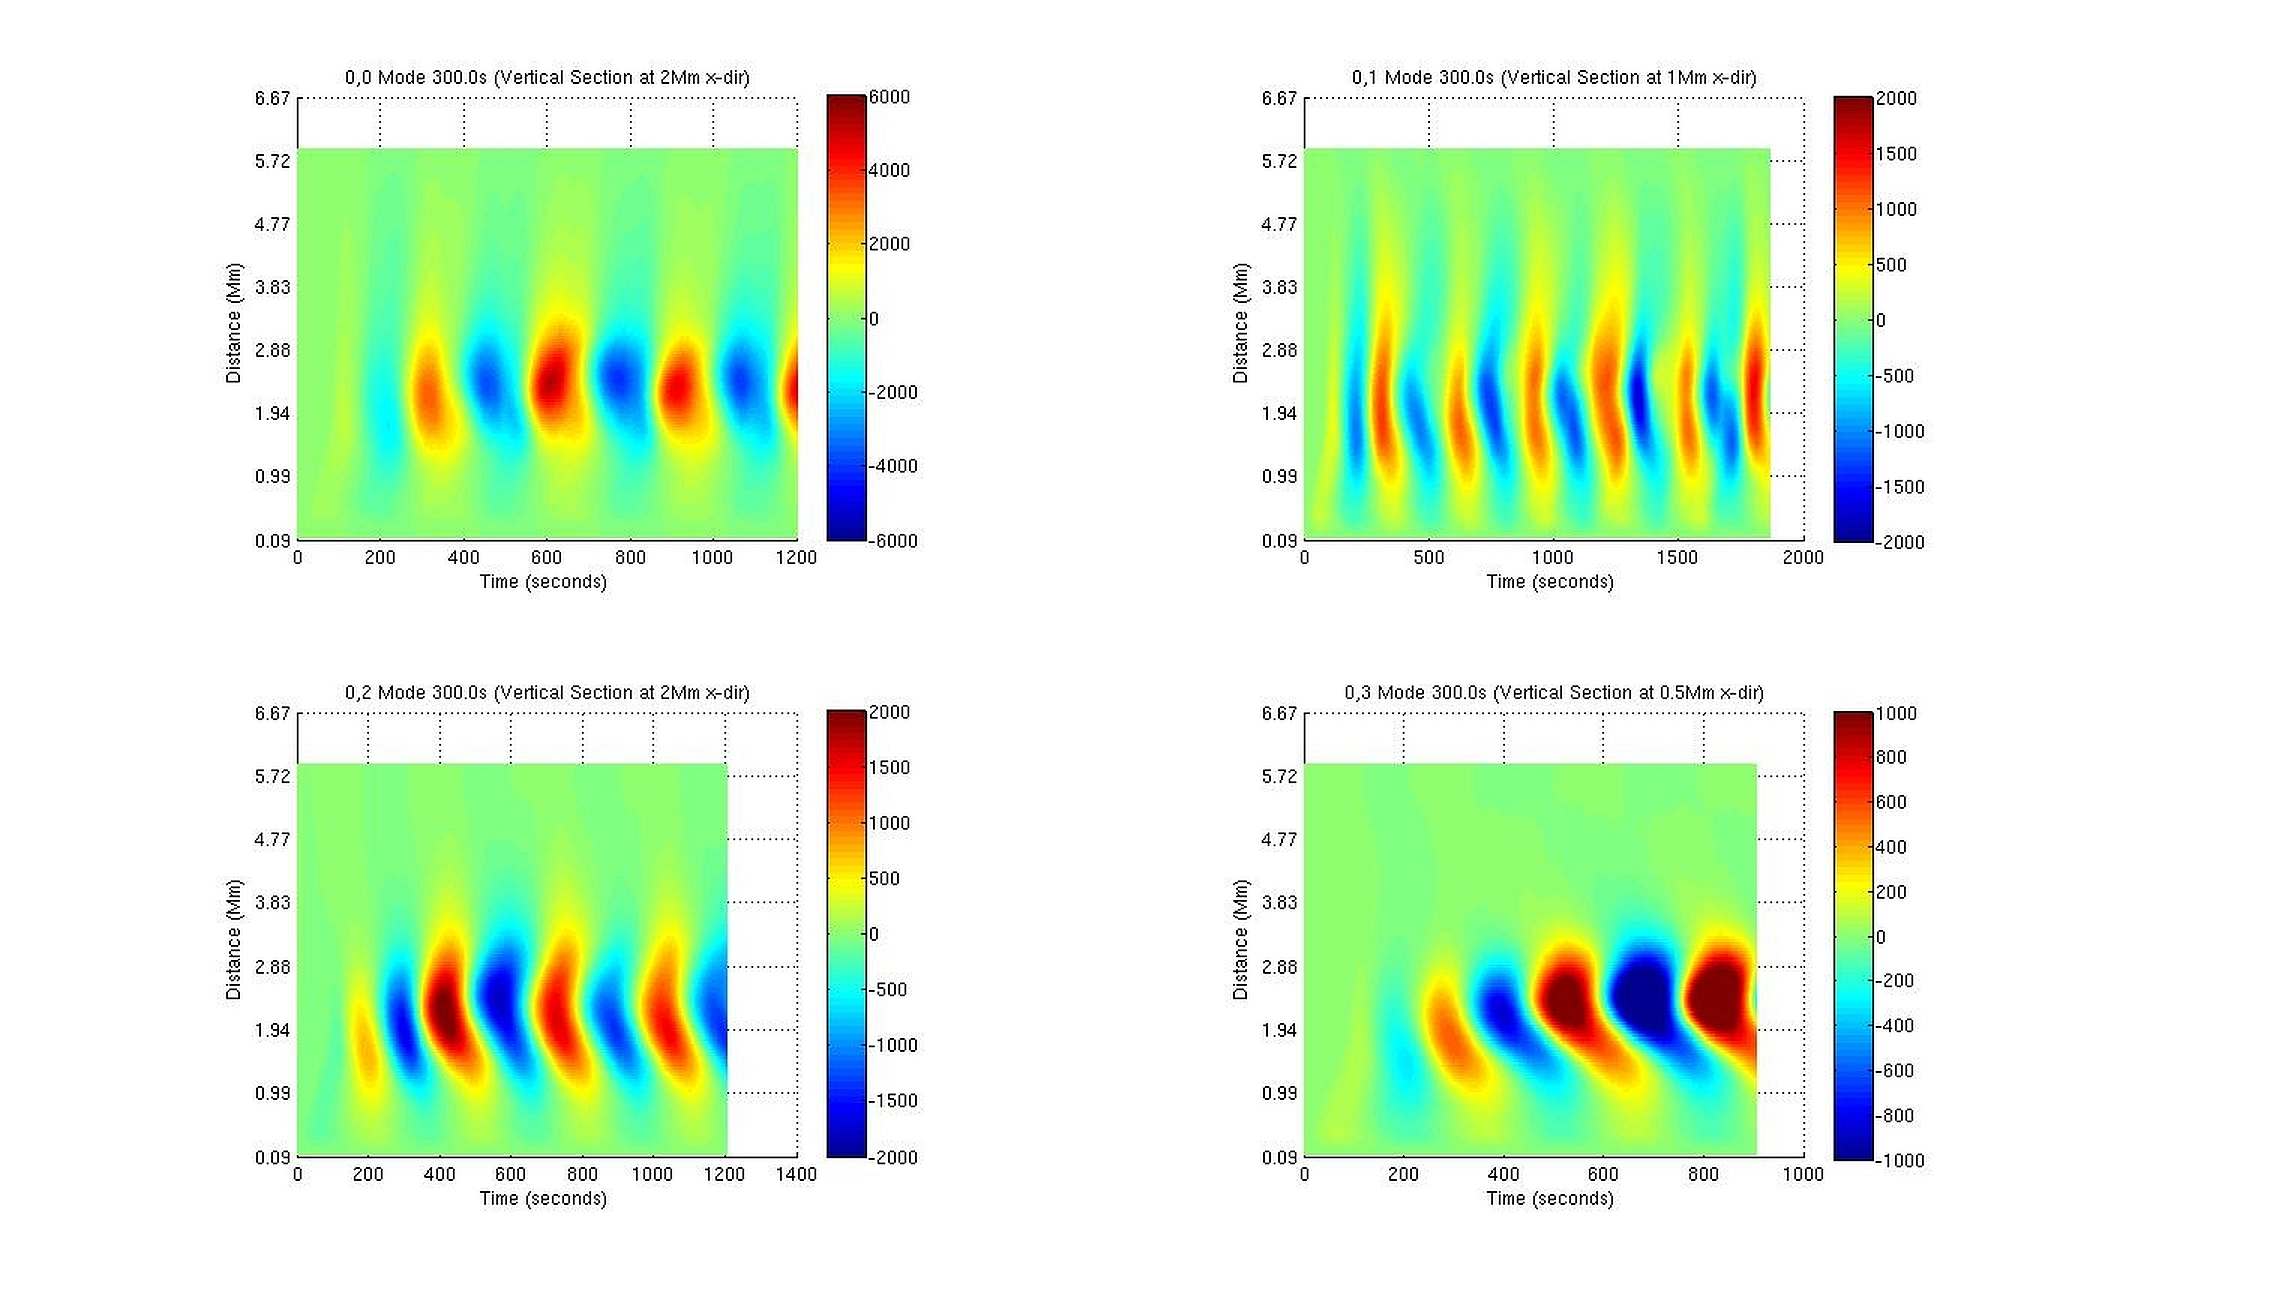
\includegraphics[scale=0.8]{imrescale/dt_300_vert_x.jpg}
\caption{Time-distance plot for the fundamental mode with the 300 s period for the z component of the velocity. $x$-direction }
\label{Fig7}
\end{figure}

%FIGURE 8 here caption:Time-distance plot for fundamental model with 180s period for the z  component of the velocity. x-direction\\

%this figure DOES not have a \label !!! i.e not shown in text !!
%\begin{figure}[h]
%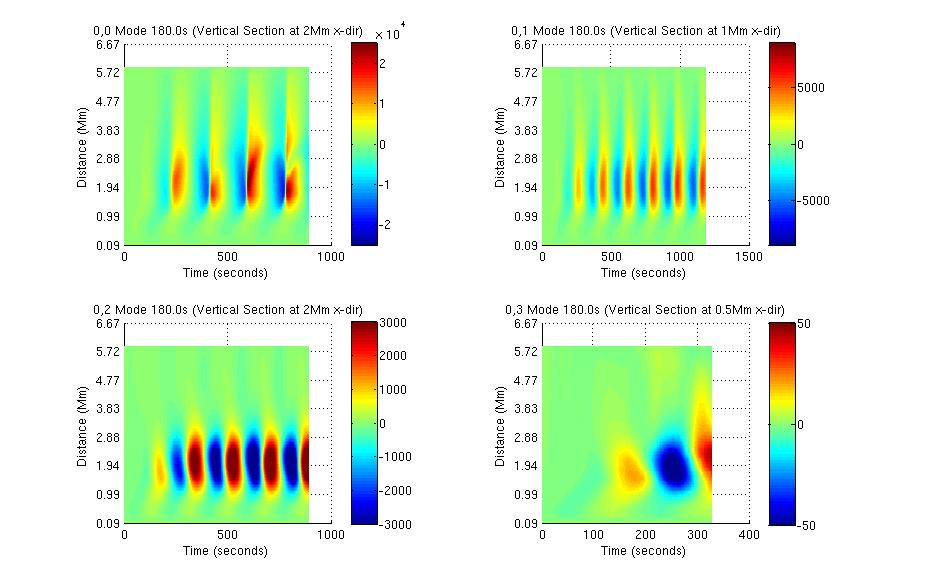
\includegraphics[scale=0.45]{imagesn/dt_180_vert_x.jpg}
%\caption{Time-distance plot for fundamental model with 180 $s$ period for the $z$ component of the velocity.  $x$-direction}
%\end{figure}


%FIGURE 9 here caption:Time-distance plot for fundamental model with 300s period for the z  component of the velocity. y-direction\\

%this figure DOES not have a \label !!! i.e not shown in text !!
%\begin{figure}[h]
%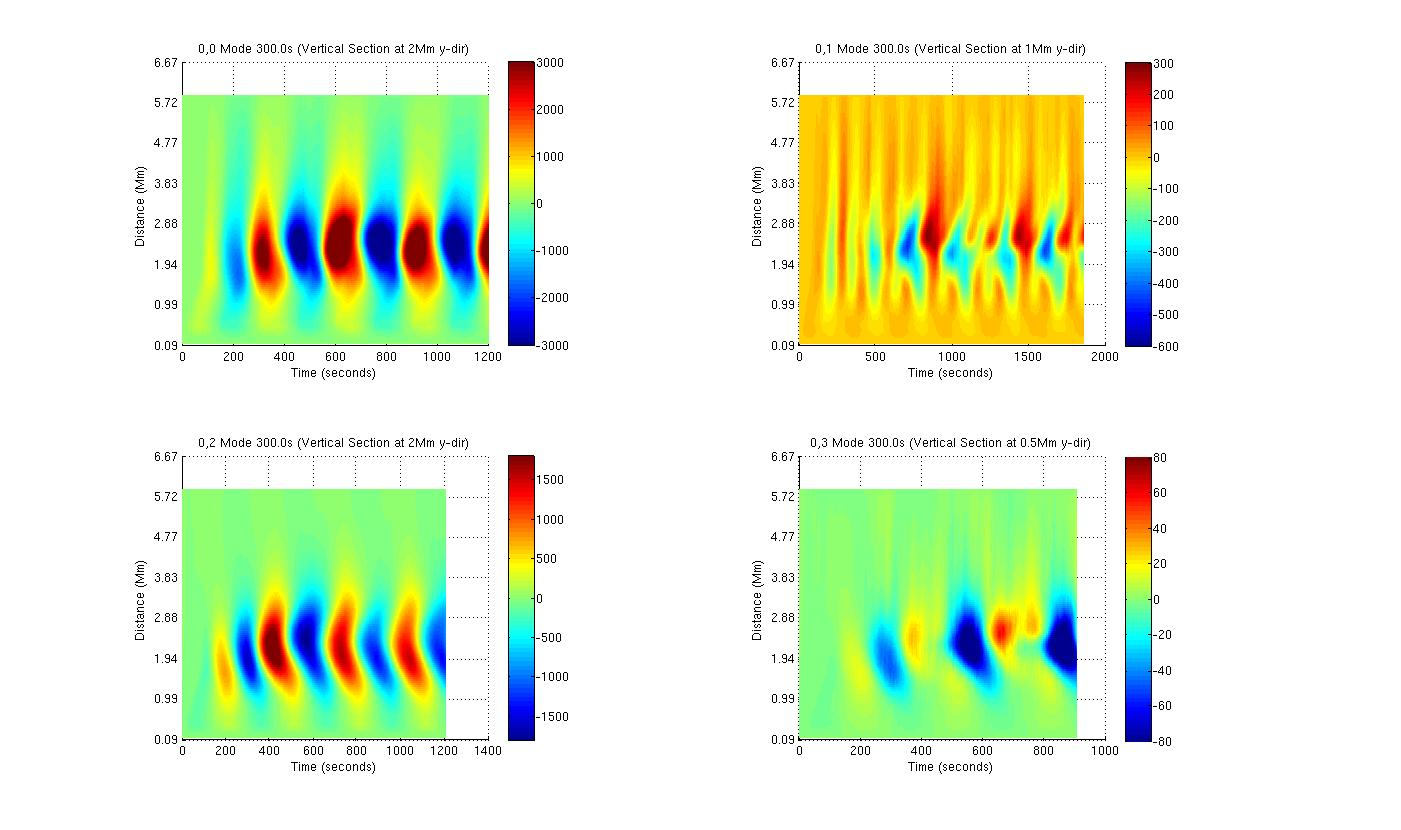
\includegraphics[scale=0.3]{imagesn/dt_300_vert_y.jpg}
%\caption{Time-distance plot for fundamental model with 300 $s$ period for the $z$ component of the velocity. $y$-direction }
%\end{figure}

%FIGURE 10 here caption:Time-distance plot for fundamental model with 180s period for the z  component of the velocity. y-direction\\

%this figure DOES not have a \label !!! i.e not shown in text !!
%\begin{figure}[h]
%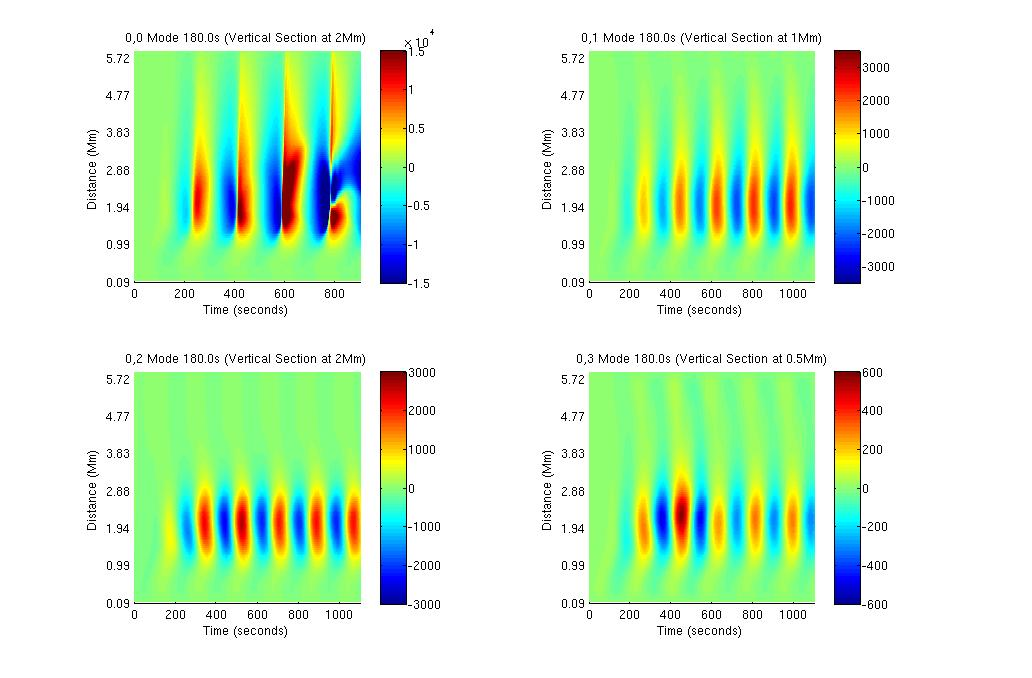
\includegraphics[scale=0.3]{imagesn/dt_180_vert_y.jpg}
%\caption{Time-distance plot for fundamental model with 180 s period for the $z$ component of the velocity.  $y$-direction}
%\end{figure}



%FIGURE 11 here caption:Time-distance plot for modes with 300s period Horizontal Section through the Chromosphere (at 1Mm) for the z  component of the velocity. x-direction\\
\begin{figure*}[h]
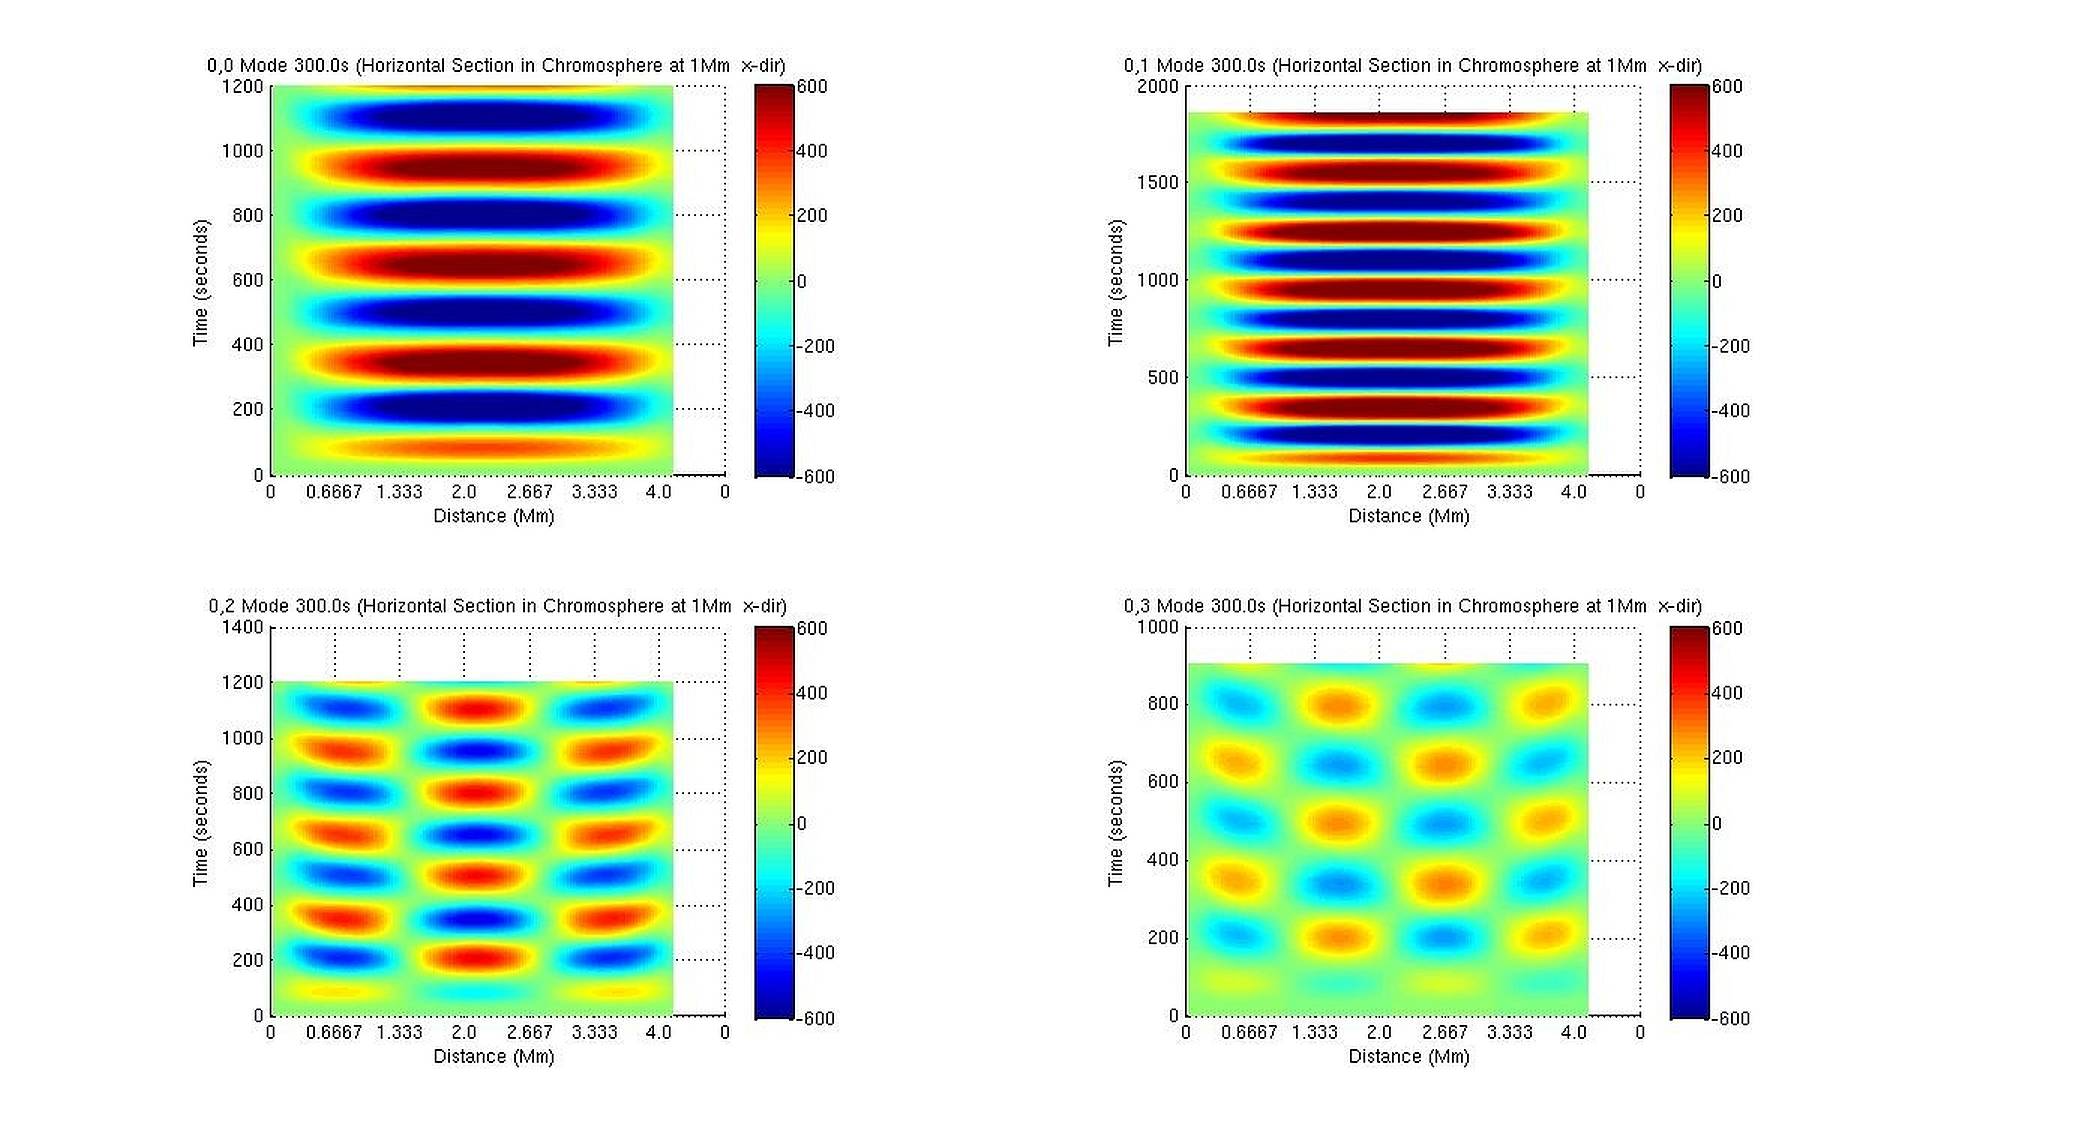
\includegraphics[scale=0.9]{imrescale/dt_300_0_0_hor_x_1Mm.jpg}
\caption{Time-distance plot for modes with 300 s period horizontal section through the chromosphere (at 1 Mm) for the $z$  component of the velocity. $x$-direction}
\label{Fig11}
\end{figure*}

%FIGURE 12 here caption:Time-distance plot for modes with 300s period Horizontal Section through the Transition Region (at 2.06Mm) for the z  component of the velocity. x-direction\\
\begin{figure*}[h]
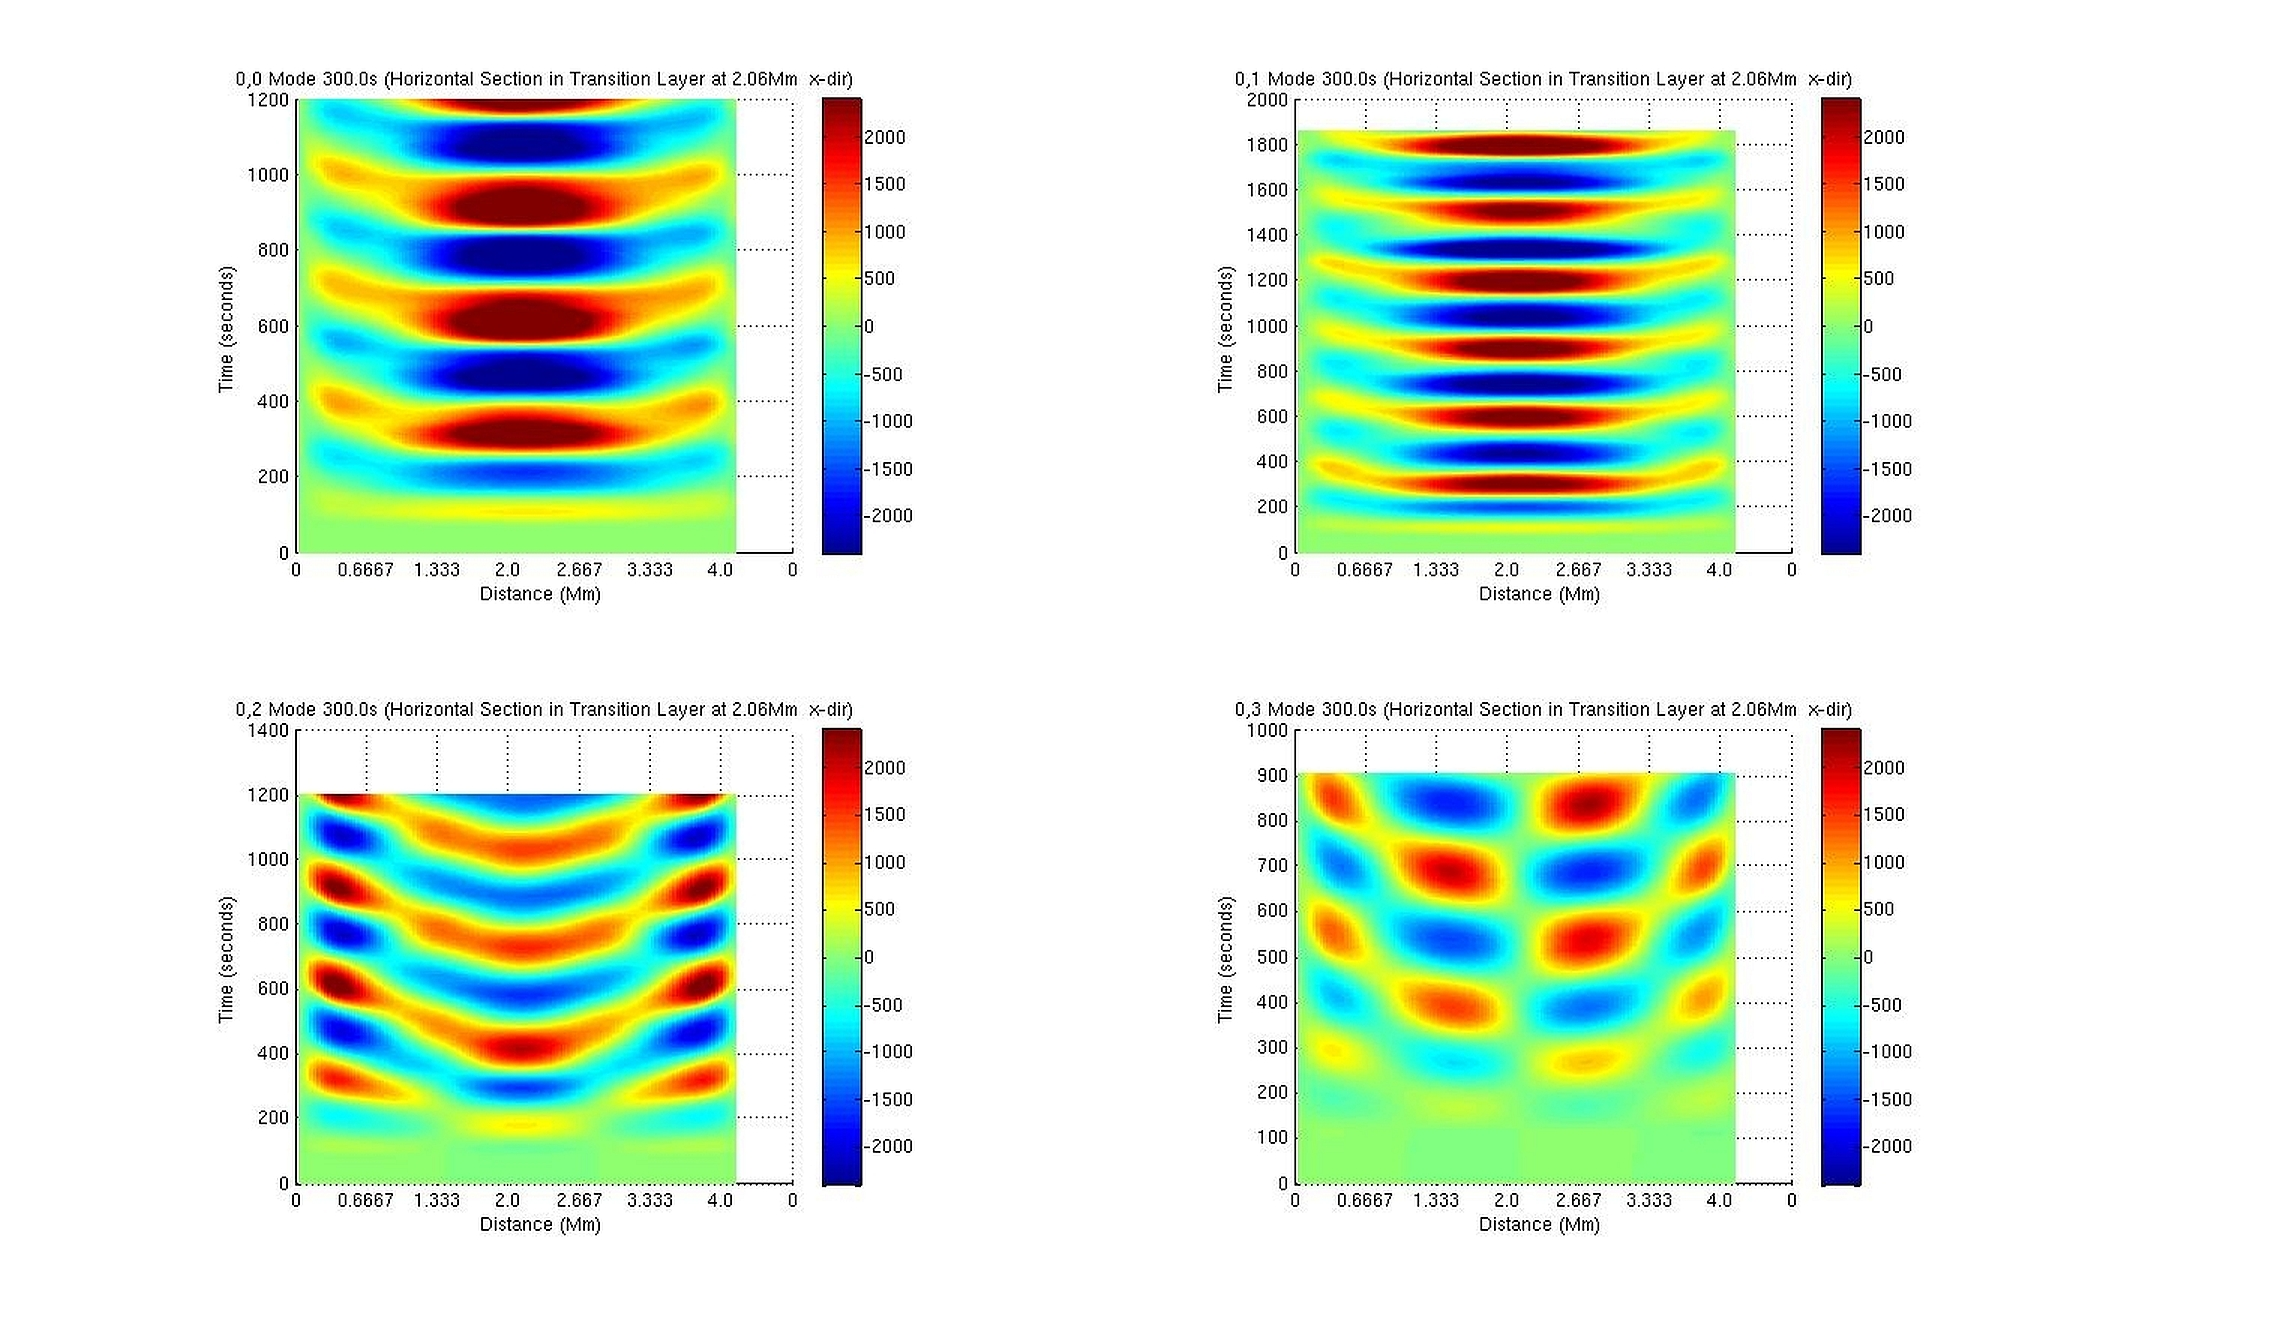
\includegraphics[scale=0.9]{imrescale/dt_300_hor_x_2p06Mm.jpg}
\caption{Time-distance plot for modes with 300 s period, horizontal section through the Transition Region (at 2.06 Mm) 
for the $z$  component of the velocity. $x$-direction}
\end{figure*}

%FIGURE 13 here caption:Time-distance plot for modes with 300s period Horizontal Section through the Transition Region (at 4.3Mm) for the z  component of the velocity. x-direction\\
\begin{figure*}[h]
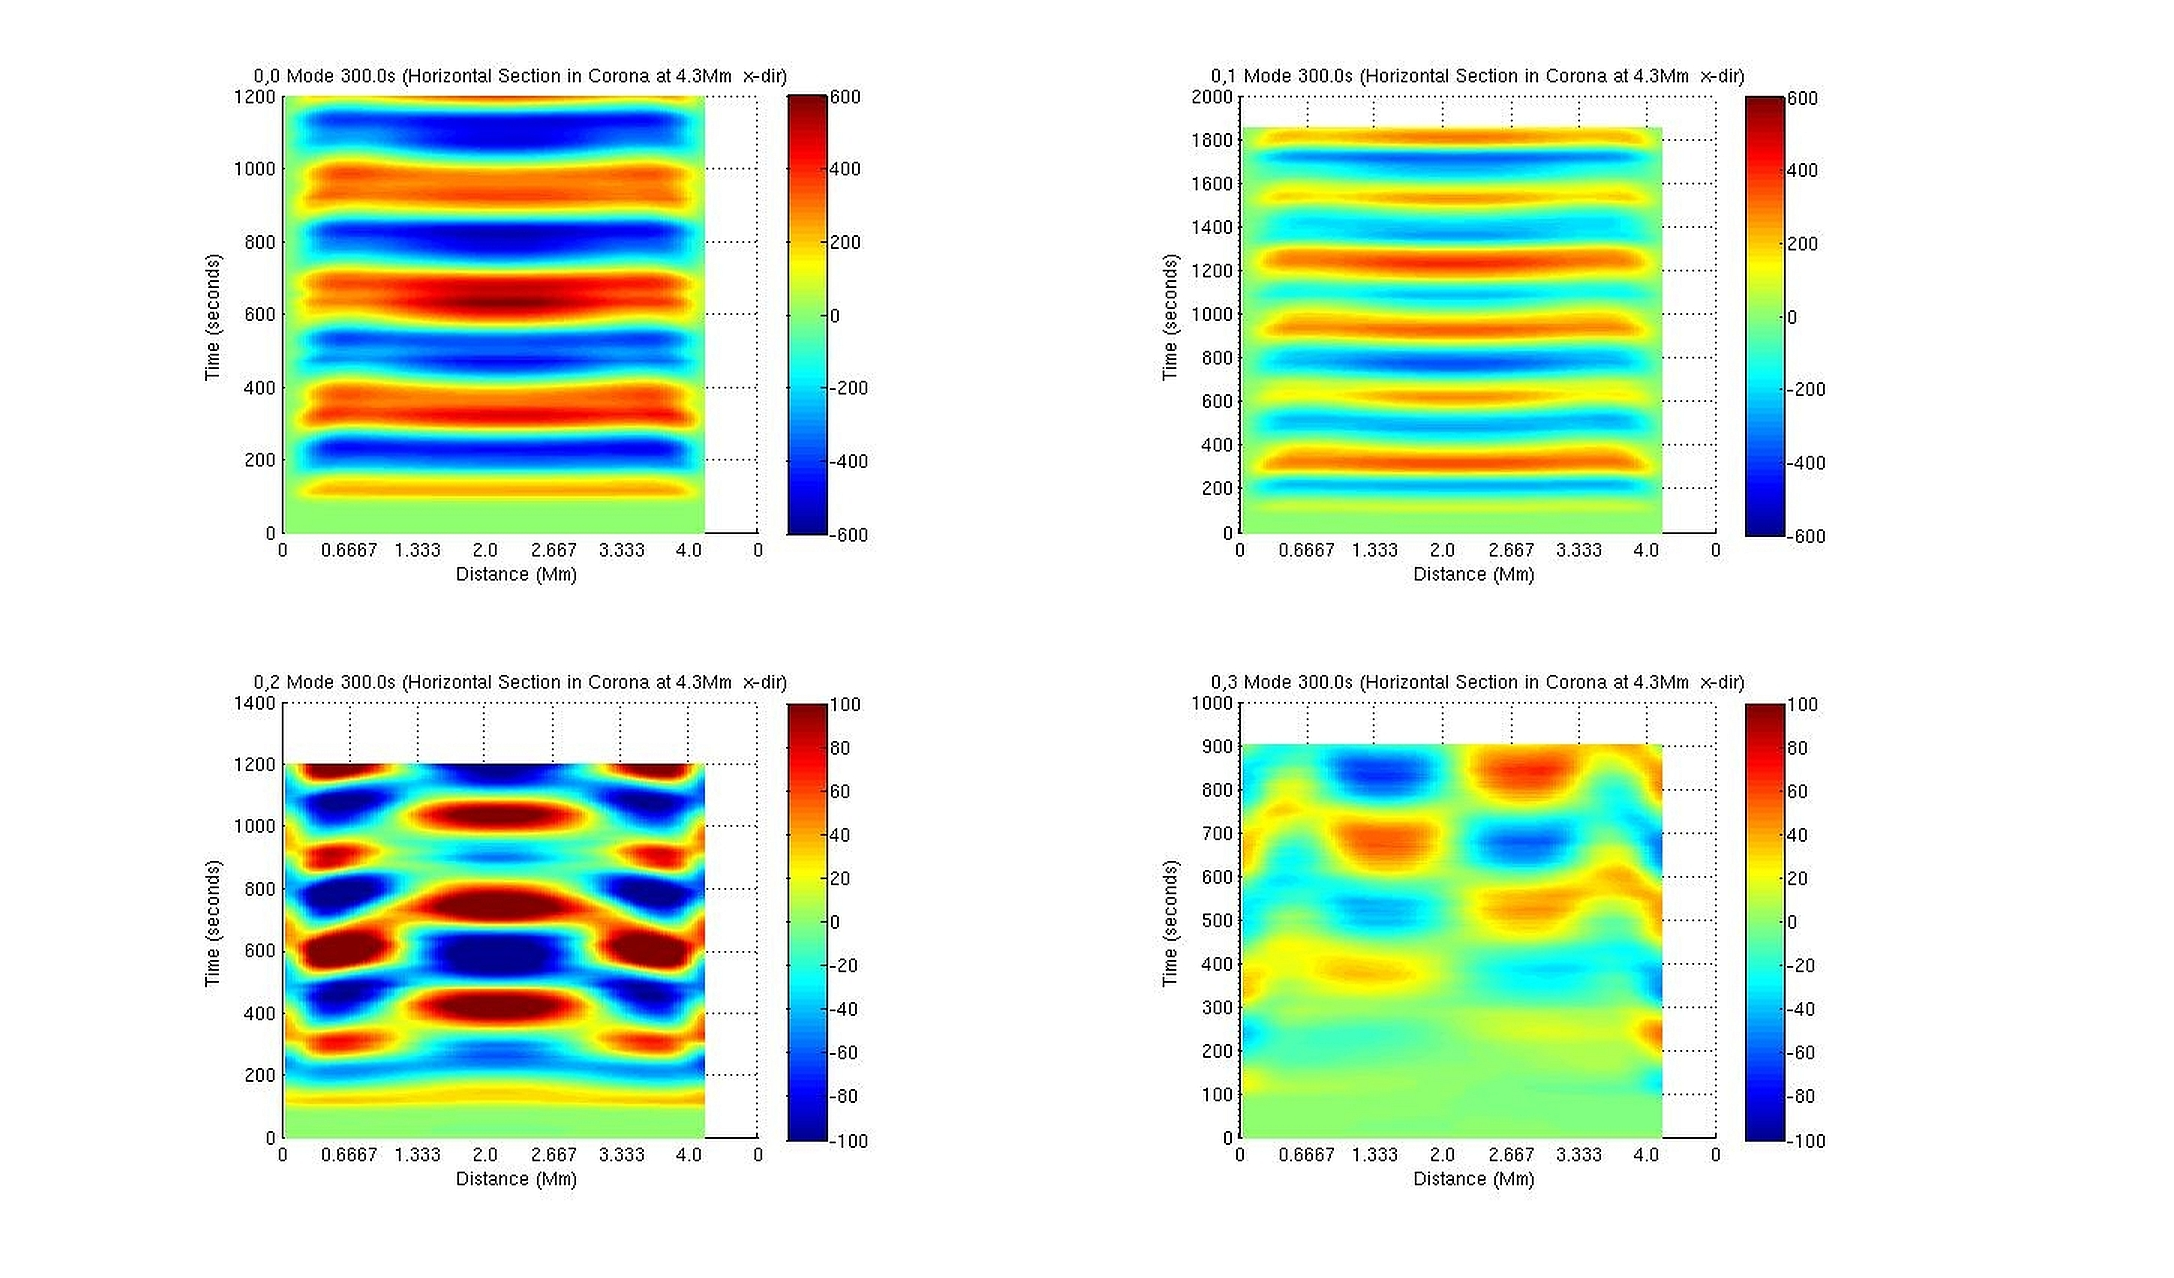
\includegraphics[scale=0.9]{imrescale/dt_300_hor_x_4p3Mm.jpg}
\caption{Time-distance plot for modes with 300 s period Horizontal Section through the Solar Corona (at 4.3 Mm) for the $z$ component of the velocity. $x$-direction}
\end{figure*}


%FIGURE 14 here caption:Time-distance plot for modes with 180s period Horizontal Section through the Chromosphere (at 1Mm) for the z  component of the velocity. x-direction\\
\begin{figure*}[h]
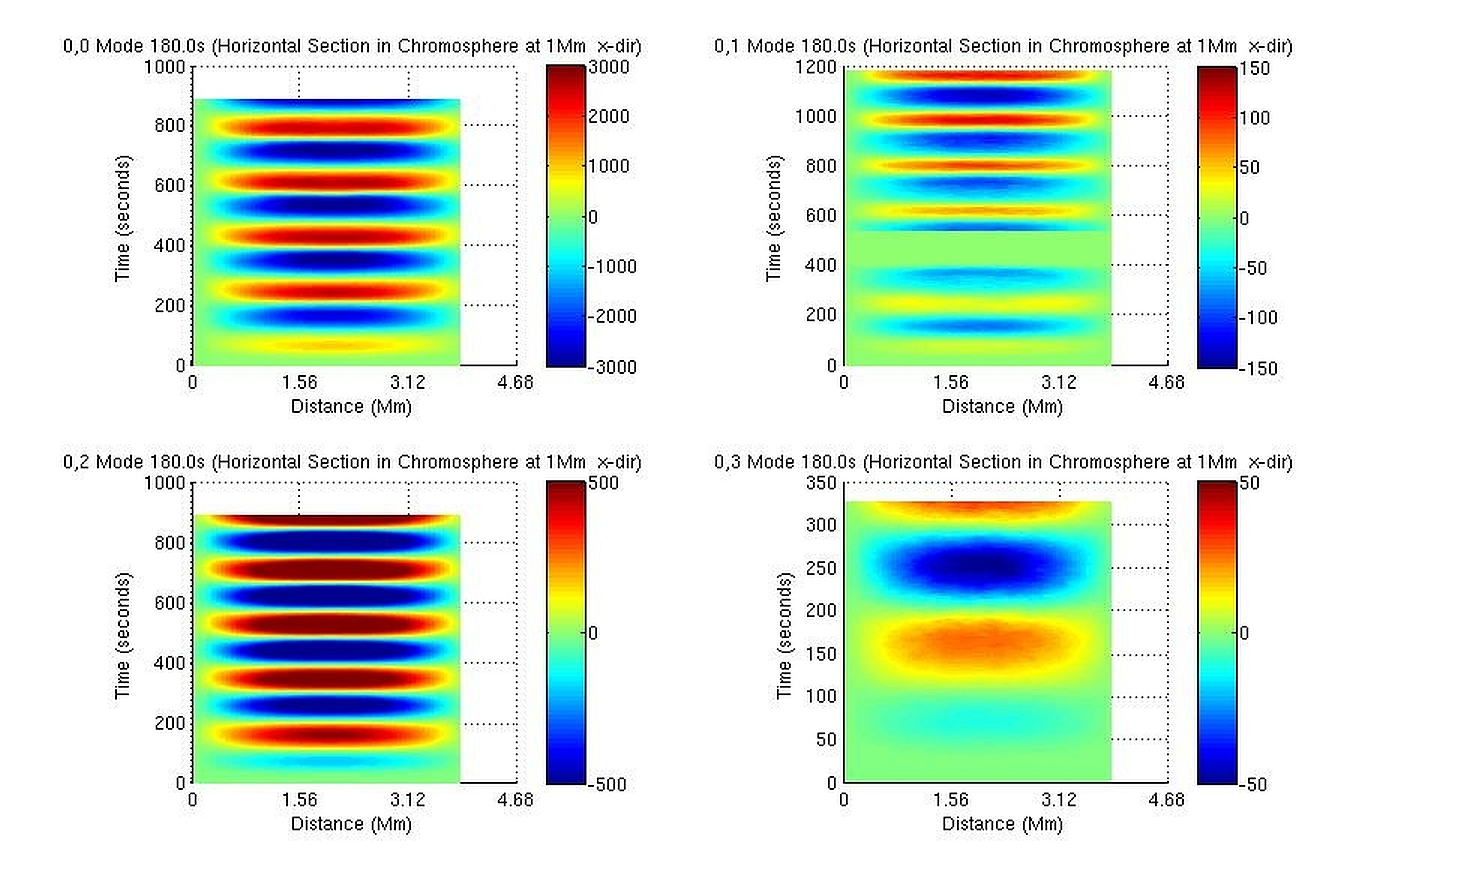
\includegraphics[scale=0.9]{imrescale/dt_180_horiz_x_1Mm.jpg}
\caption{Time-distance plot for modes with 180 s period Horizontal Section through the Chromosphere (at 1 Mm) for the $z$ component of the velocity. $x$-direction}
\label{Fig14}
\end{figure*}

%FIGURE 15 here caption:Time-distance plot for modes with 180s period Horizontal Section through the Transition Region (at 2.06Mm) for the z  component of the velocity. x-direction\\
\begin{figure*}[h]
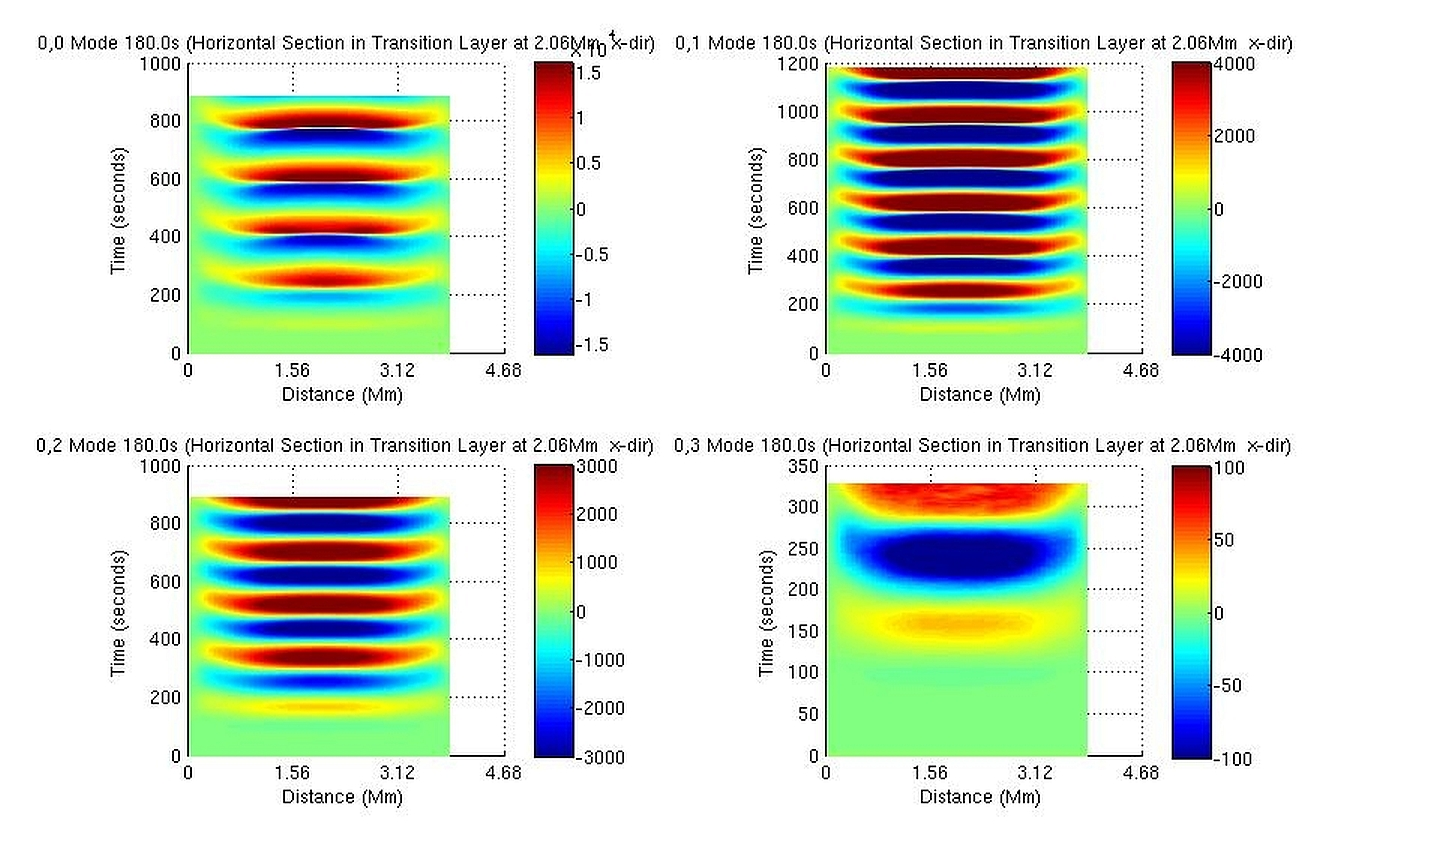
\includegraphics[scale=1]{imrescale/dt_180_horiz_x_2p06Mm.jpg}
\caption{Time-distance plot for modes with 180 s period Horizontal Section through the Transition Region (at 2.06 Mm) for the $z$  component of the velocity. $x$-direction}
\label{Fig15}
\end{figure*}

%FIGURE 16 here caption:Time-distance plot for modes with 180s period Horizontal Section through the Transition Region (at 4.3 Mm) for the z  component of the velocity. x-direction\\
\begin{figure*}[h]
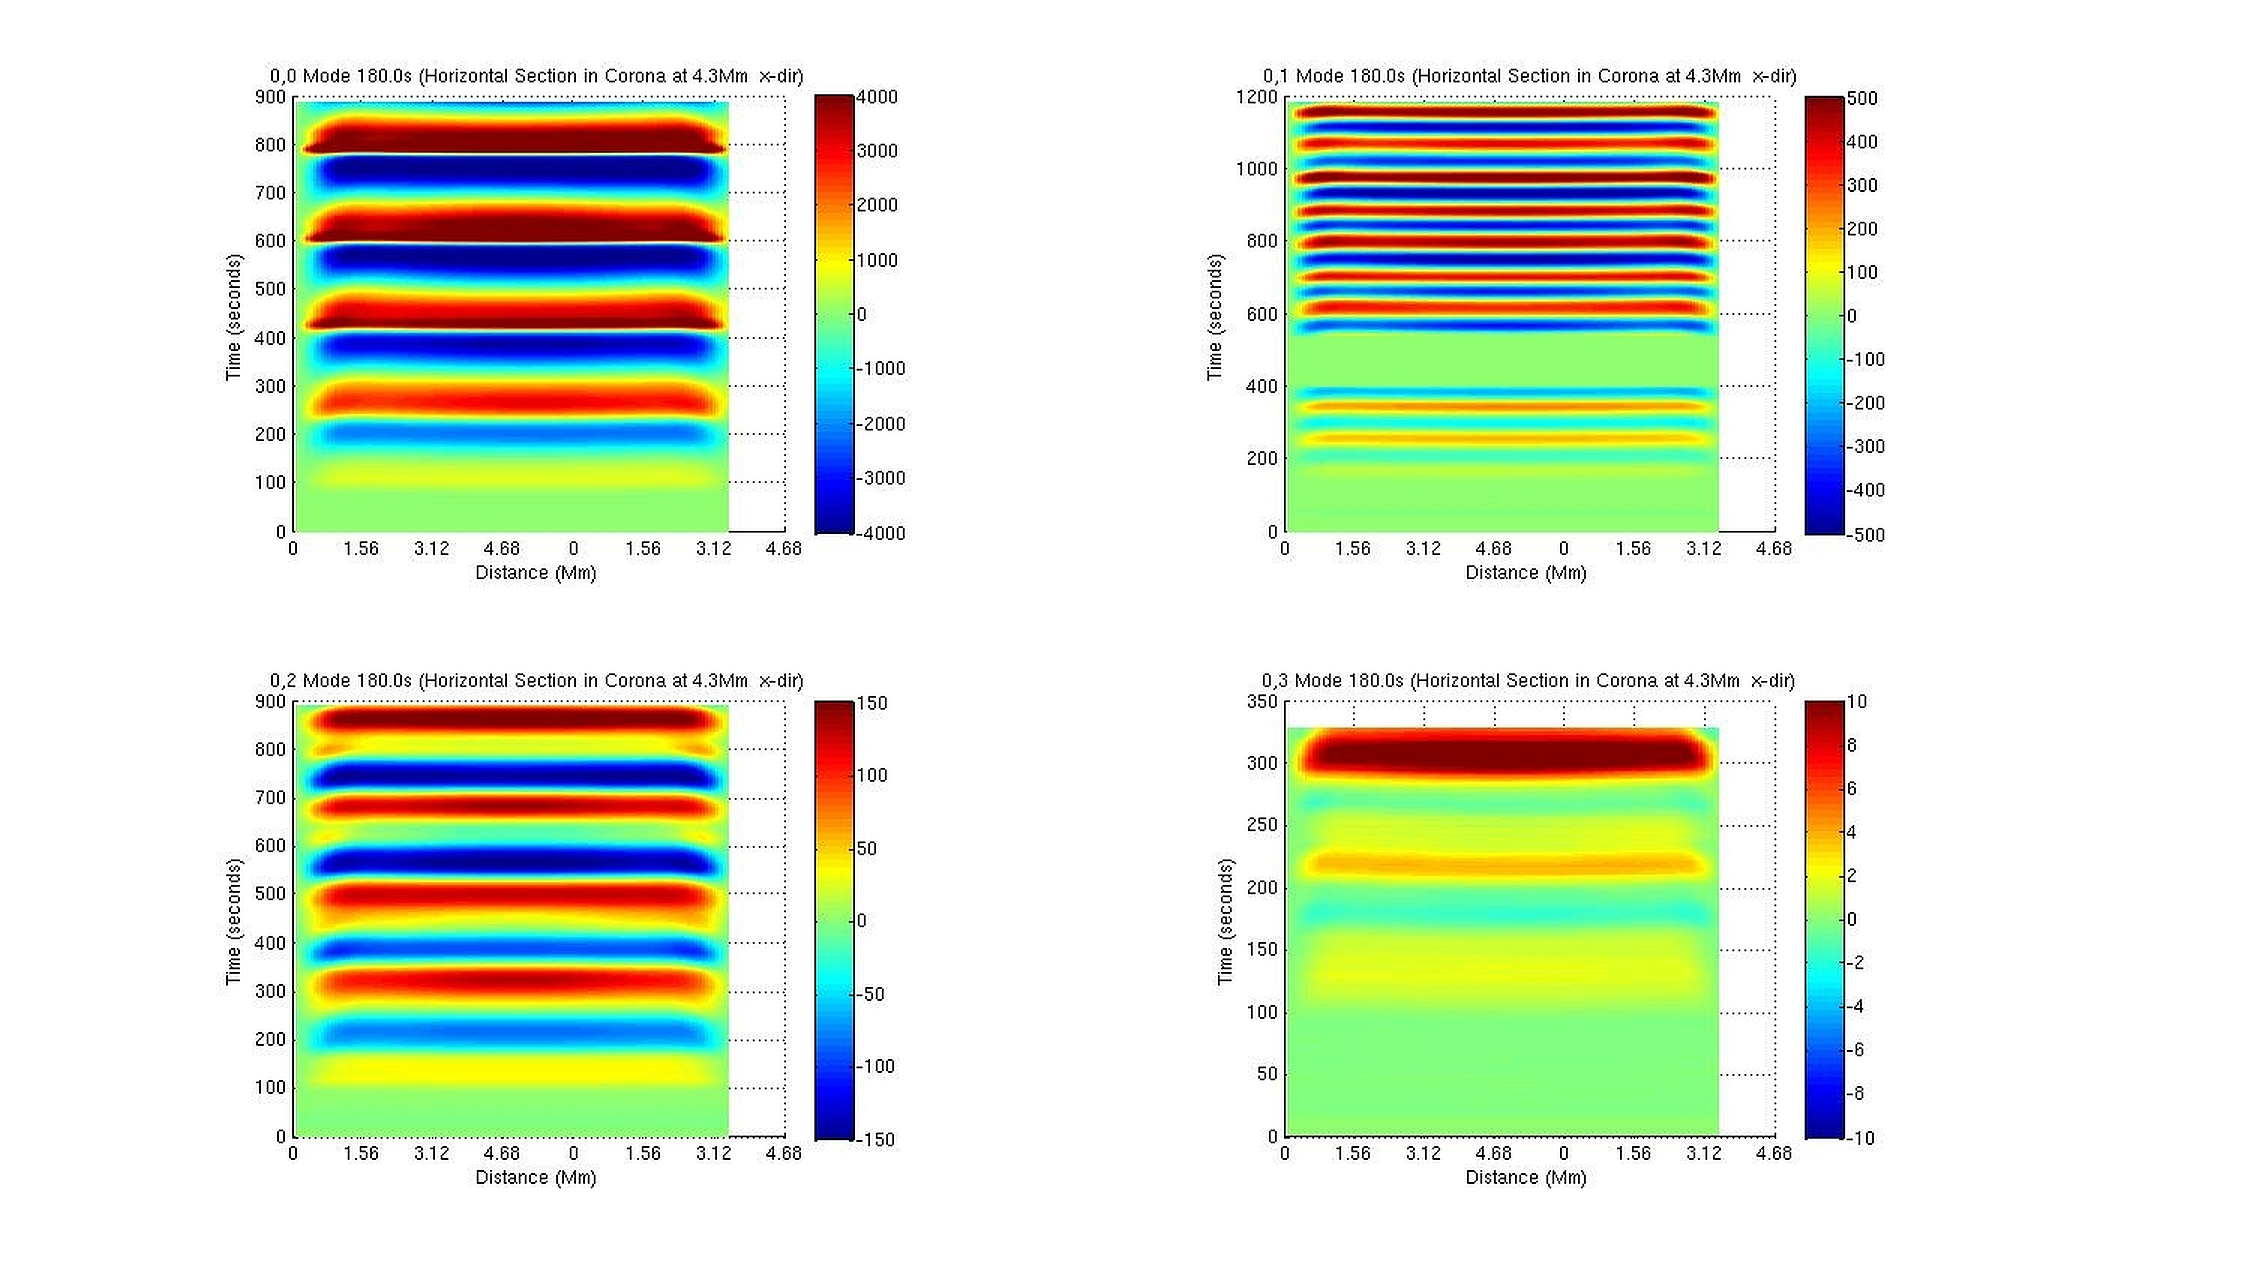
\includegraphics[scale=1]{imrescale/dt_180_horiz_x_4p3Mm.jpg}
\caption{Time-distance plot for modes with 180 s period Horizontal Section through the Solar Corona (at 4.3 Mm) for the $z$ component of the velocity. $x$-direction}
\label{Fig16}
\end{figure*}

Using Equation (\ref{e11}), we compute the energy flux integral for the range of driver frequencies, modes and at different atmospheric heights. Figure (\ref{Fig17}) shows the variation of the energy flux ratio.  Figure \ref{Fig18} and \ref{Fig19} show the energy ratios for the different modes. Fitting  the  data for the $(0, 0)$ mode against the power law shown in equation (\ref{energyfluxpowerlaw}) gives the values shown in Table \ref{Table3}, we obtain power laws for the energy flux at 5.5Mm and the energy flux at 2Mm. \ref{Fig20} shows a comparison of the energy flux ratio for the $(0,0)$-mode with the observational power law ratio from the results of  \citet{Ireland2015}. For the simulation results we compute the ratio of the energy flux at 5.5Mm to the energy flux at 2Mm. For the observational data we compute the ratio of the power laws for the results at 193{\AA} and the results at 193{\AA}. Six pairs of period and flux values were used for the fitting procedure. The results suggest that our simulated data give rise to a flat power spectrum as opposed to the power law suggested by \citet{Ireland2015}.






\begin{equation}
P(z)= aT^{b}+c,
\label{energyfluxpowerlaw}
\end{equation}
\begin{table*}
\centering
\begin{tabular}{cccc}
\hline
   &  ((00) mode at 5.5Mm) &  ((00) mode at 2Mm) & Ireland (171{\AA}) & Ireland (193{\AA}) \\
\hline
a & -0.000805 &-0.003733 &  $10^{0.57}$ & $10^{-0.1}$ \\
\hline
b & 2.732  & 2.716 & 1.72 & 2.2 \\
\hline
c & 1.096x$10^{4}  & 4.724x$10^{4} & $10^{-3}$ & $10^{-3.52}$ \\
\hline
\end{tabular} 
\caption{ Power law coefficients for relationship between power and time-period of atmospheric oscillation.}
\label{Table3}
\end{table*}



The Tables \ref{Table00mode},\ref{Table01mode},\ref{Table02mode} and \ref{Table03mode} show the resulting values of the energy flux ratio from the simulations at different heights. The energy is the ratio of the enrgy flux at a given height to the energy flux at the location of the driver. All the modes for the driver periods 180 and 300 s are shown as a bar chart in Figures (\ref{Fig18}) and (\ref{Fig19}) see also tables \ref{Table180mode} and \ref{Table300mode}. For both the 180 and 300 s drivers it can be seen that the even modes make the strongest contribution in the corona. The results plotted in Figure (\ref{Fig20}) indicate the ratio of the energy flux for models delivering the same quantity of energy to the energy flux for models where the driver amplitude is kept fixed. With the exception of the fundamental mode, the ratios appear to be constant for all frequencies suggesting the possibility of using the scaling relation to compute the energy flux for different frequencies and modes.  
\begin{figure}[h]
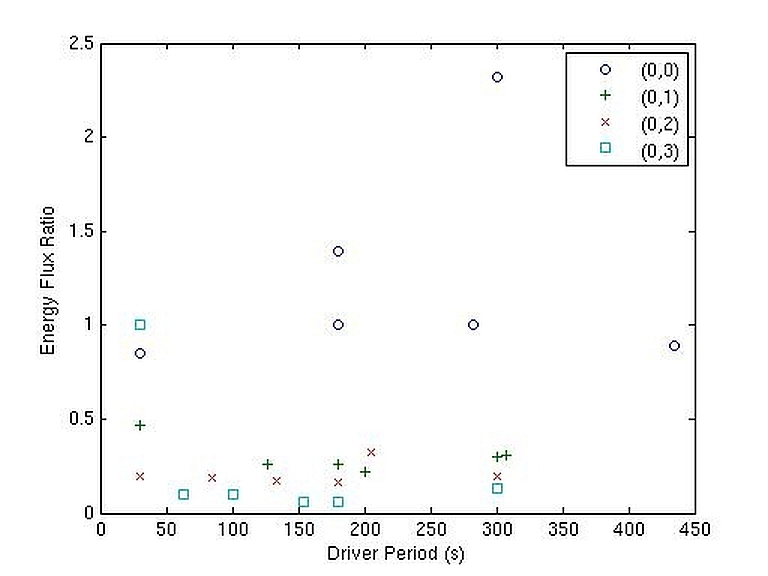
\includegraphics[scale=3]{imrescale/ratio_varoverconst_eflux_vperiod_for_modes_5p5Mm.jpg}
\caption{Variation of energy flux ratio at height of 5.5 Mm for a solar atmosphere excited with a $p$-mode driver providing the same amount of energy for all driver modes and periods}
\label{Fig20}
\end{figure}





\begin{figure}[t]
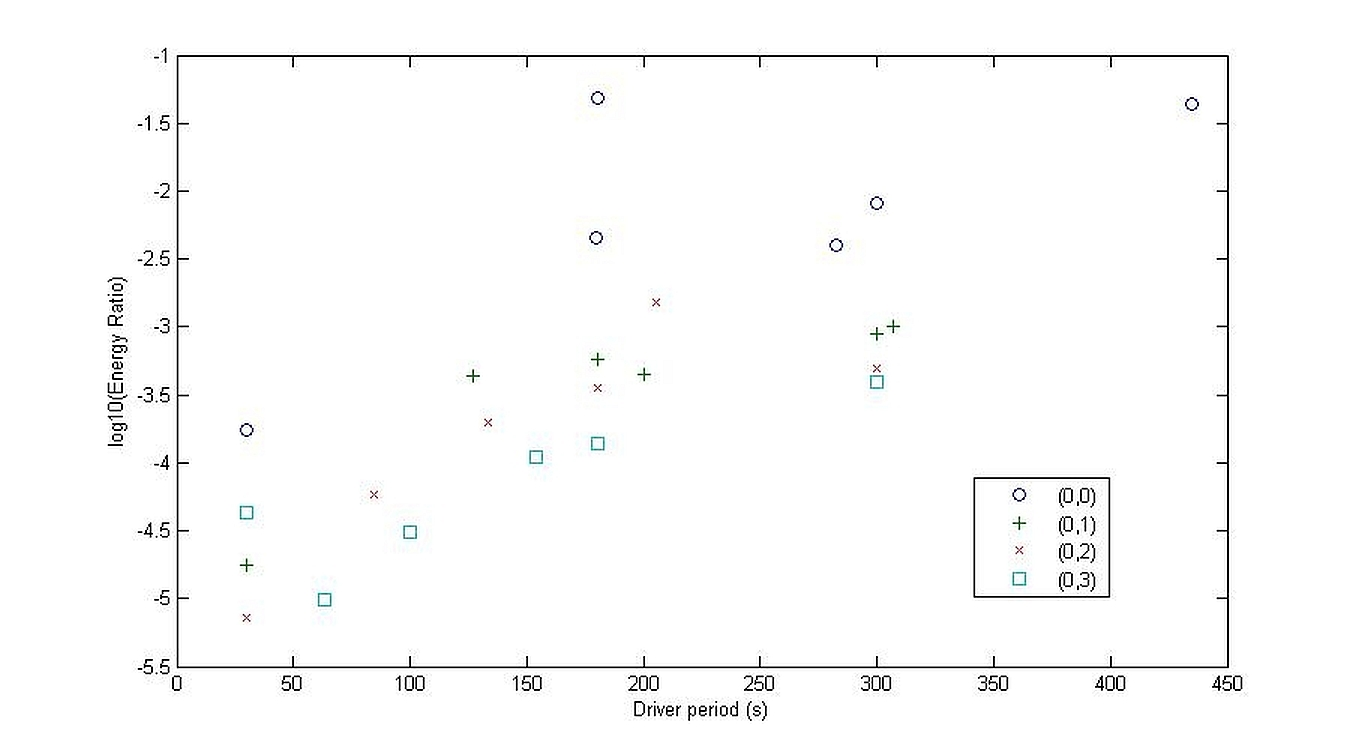
\includegraphics[scale=2]{imrescale/ratio_varoverdrve_eflux_vperiod_for_modes_5p5Mm.jpg}
\caption{Variation of energy flux ratio with the driver energy at height of 5.5 Mm for a solar atmosphere excited with a {\it p}-mode driver of fixed amplitude}
\label{Fig17}
\end{figure}


\begin{figure}[t]
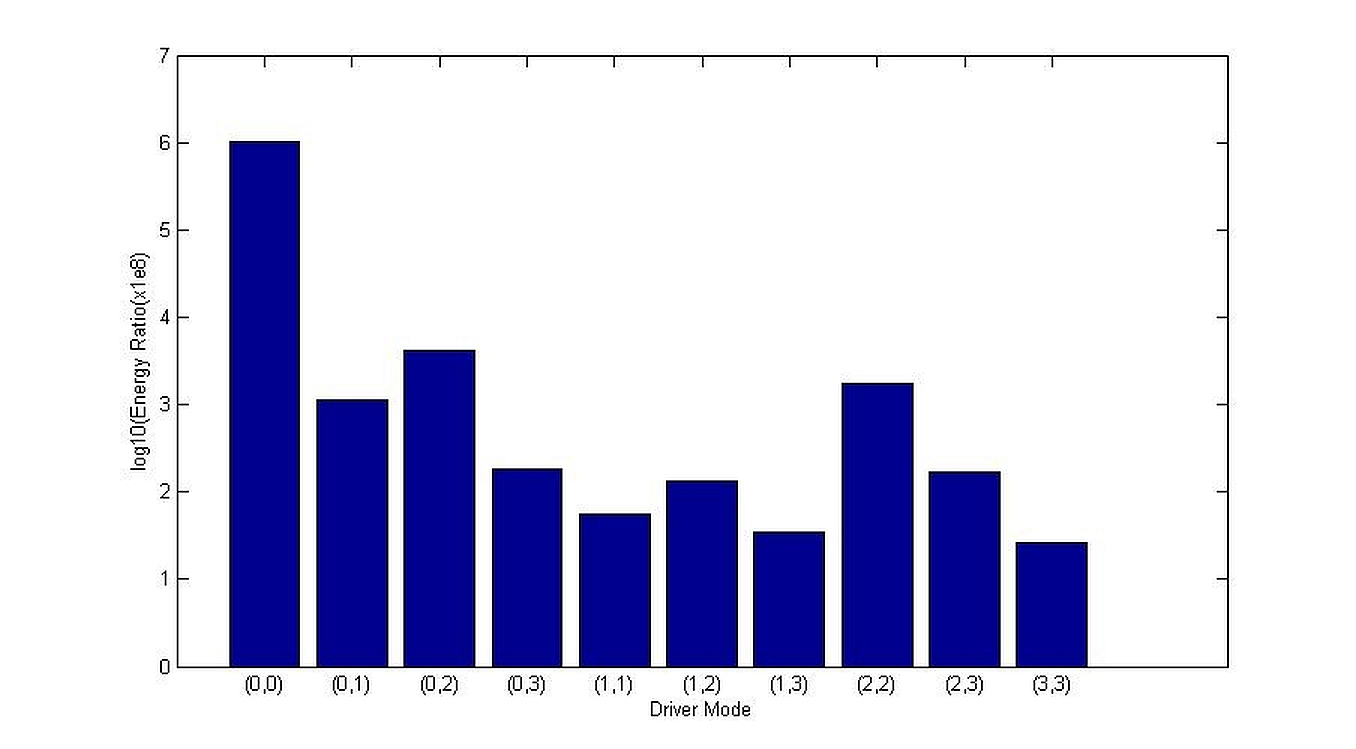
\includegraphics[scale=2]{imrescale/ratio_varoverdrve_eflux_vperiod_forallmodes_180s_5p5Mm.jpg}
\caption{Variation of energy flux ratio at a height of 5.5 Mm for a solar atmosphere excited with 180 s {\it p}-mode driver located 
at height of 50 km}
\label{Fig18}
\end{figure}

\begin{figure}[t]
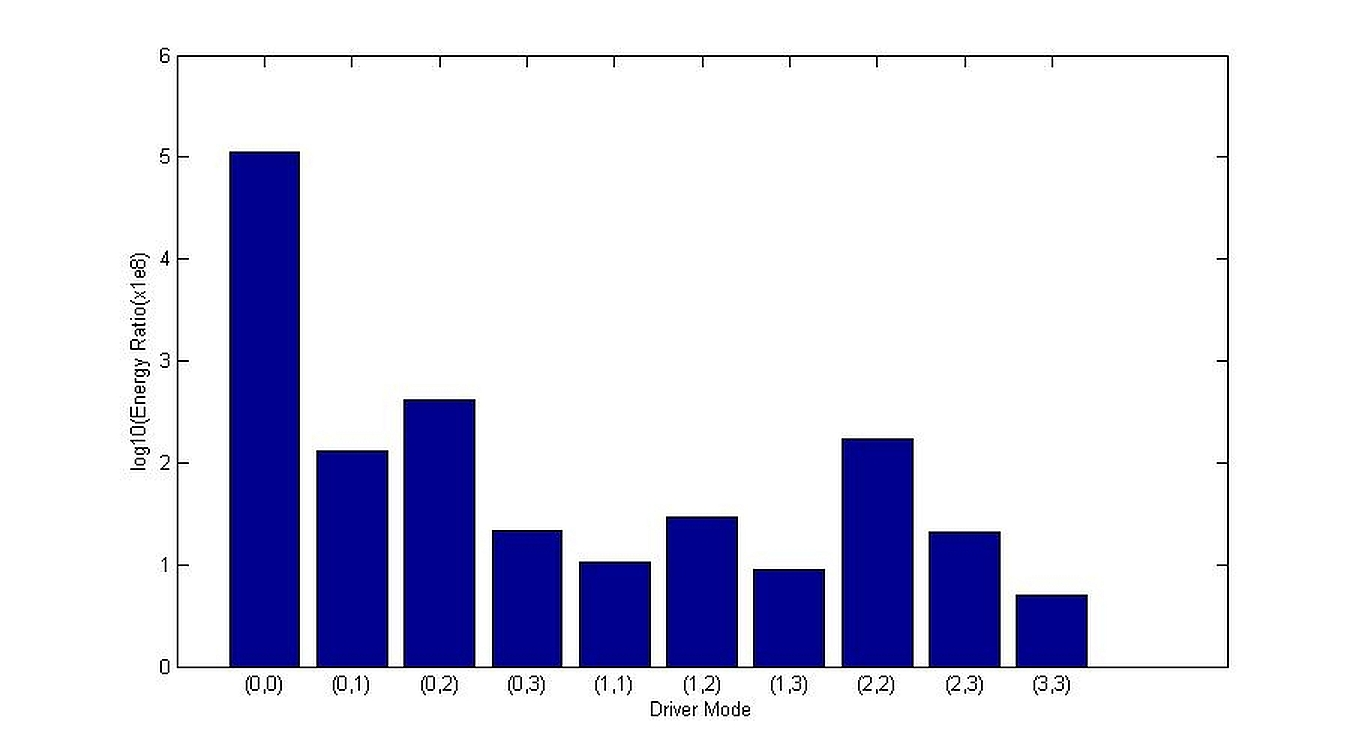
\includegraphics[scale=2]{imrescale/ratio_varoverdrve_eflux_vperiod_forallmodes_300s_5p5Mm.jpg}
\caption{Variation of energy flux ratio at height of 5.5 Mm for a solar atmosphere excited with a 300 s $p$-mode driver 
located at a height of 50 km}
\label{Fig19}
\end{figure}


\begin{figure}[t]
\includegraphics[scale=4]{imrescale/fig20_powerlaw_comparison.jpg}
\caption{Comparison of the energy flux ratio for the $(0,0)$-mode with the observational power law ratio from the results of  \citet{Ireland2015}. For the simulation results we compute the ratio of the energy flux at $5.5Mm$ to the energy flux at $2Mm$. For the observational data we compute the ratio of the power laws for the results at 193{\AA} and the results at 193{\AA}.}
\label{Fig20}
\end{figure}




\section{Conclusions}

In this paper, motivated by the reported plentiful intensity oscillations at various layers of the solar atmosphere from low chromosphere to corona detected by the currently available suite of high-resolution space-based instrumentation (e.g. SDO), we embarked on a simple model to investigate whether these oscillations may be linked to the global solar acoustic oscillations of the photosphere. We approximated the solar atmosphere by a purely hydrodynamic VAL III-type of equilibrium. The perturbations mimicking the photospheric coherence pattern of a range of periods of $p$-mode oscillations were implemented at the lower boundary of the simulation box. The perturbations themselves were only allowed in the vertical (i.e. radial) direction. Therefore waves were propagating by large along the $z$-axis from the photosphere into the lower solar corona. The wave propagation was followed and their frequency spectrum derived and compared to observed frequency spectra.

Our results support the notion that solar global oscillations may be a driver for a range of global dynamical phenomena 
resulting in chromospheric and low coronal Doppler and intensity oscillations which, after all, may contribute to the non-thermal energy present in the solar atmosphere. We would like to emphasise that these upper atmospheric ubiquitous wave phenomena may not arise solely from the photospheric $p$-modes. On the contrary, a range of sources including, turbulent motions from convective cells, local nano-flares, small-scale Kelvin-Helmholtz instabilities, or continuous reconnection events in the magnetic carpet may contribute to their excitation. 

Among others, we found that
   \begin{enumerate}
      \item there is consistency between the frequency-dependence of the energy flux in the numerical simulations and power 
      flux measurements obtained from SDO;
      \item energy propagation into the mid- to upper-atmosphere of the quiet Sun occurs for a range of frequencies and may explain observed intensity oscillations for periods greater than the well known 3-minute and 5-minute oscillations; 
      \item energy flux propagation into the lower solar corona is strongly dependent on the particular wave modes;
 \item agreement between the energy flux predictions of our numerical simulations and that of the two layer 
      Klein-Gordon model supports our interpretation of the interaction of solar global oscillations with the solar atmosphere.
   \end{enumerate}

An important caveat of the present work is the modelling of the active response of the atmospheric magnetic field. Although the plasma-$\beta$ is very large in the low corona, this approximation may serve an appropriate initial insight, nevertheless one needs to relax this condition and analyse how perhaps the mean magnetic field itself would change the coupling of the global solar acoustic modes to the overlaying magnetised atmosphere. Here, an interesting question would be to investigate whether slow or fast MHD waves are the key stakeholders in the re-distribution of the convective kinetic energy.  

\section{Acknowledgements}
 The authors thank P. H. Keys for providing the wavelet tools to analyse the related SDO data, and, the Science and Technology Facilities Council (STFC), UK for the support they received. 
VF thanks the Royal Society-Newton Mobility Grant and Newton Fund MAS/CONACyT Mobility
Grants Program for the support received. RE acknowledges the support received from the the Royal Society (UK). 
We acknowledge Corporate Information and Computing Services at The University of Sheffield for the provision of the High Performance Computing Service.

%\begin{thebibliography}{}

% \bibitem[Names(Year)]{label} or \bibitem[Names(Year)Long names]{label}.
% (\harvarditem{Name}{Year}{label} is also supported.)
% Text of bibliographic item

%\bibliographystyle{elsarticle-num-names}
\bibliographystyle{elsarticle-harv}
%\bibliographystyle{unsrt}
%\bibliographystyle{plainnat}
\bibliography{ASR_v1}
%\begin{thebibliography}{XXX}
%\end{thebibliography}

%\end{thebibliography}









\end{document}
